% ****************************************************************************************
% ************************      ANALISIS VECTORIAL            ****************************
% ****************************************************************************************


% =======================================================
% =======         HEADER FOR DOCUMENT        ============
% =======================================================
    % *********   DOCUMENT ITSELF   **************
    \documentclass[12pt, fleqn]{report}                             %Type of docuemtn and size of font and left eq
    \usepackage[margin=1.2in]{geometry}                             %Margins and Geometry pacakge
    \usepackage{ifthen}                                             %Allow simple programming
    \usepackage{hyperref}                                           %Create MetaData for a PDF and LINKS!
    \usepackage{pdfpages}                                           %Create MetaData for a PDF and LINKS!
    \hypersetup{pageanchor=false}                                   %Solve 'double page 1' warnings in build
    \setlength{\parindent}{0pt}                                     %Eliminate ugly indentation
    \author{Oscar Andrés Rosas & Alan Enrique Ontiveros Salazar}    %Who I am

    % *********   LANGUAJE AND UFT-8   *********
    \usepackage[spanish]{babel}                                     %Please use spanish
    \usepackage[utf8]{inputenc}                                     %Please use spanish - UFT
    \usepackage[T1]{fontenc}                                        %Please use spanish
    \usepackage{textcmds}                                           %Allow us to use quoutes
    \usepackage{changepage}                                         %Allow us to use identate paragraphs
    \usepackage{anyfontsize}                                        %All the sizes

    % *********   MATH AND HIS STYLE  *********
    \usepackage{ntheorem, amsmath, amssymb, amsfonts}               %All fucking math, I want all!
    \usepackage{mathrsfs, mathtools, empheq}                        %All fucking math, I want all!
    \usepackage{centernot}                                          %Allow me to negate a symbol
    \decimalpoint                                                   %Use decimal point

    % *********   GRAPHICS AND IMAGES *********
    \usepackage{graphicx}                                           %Allow to create graphics
    \usepackage{float}
    \usepackage{wrapfig}                                            %Allow to create images
    \graphicspath{ {Graphics/} }                                    %Where are the images :D

    % *********   LISTS AND TABLES ***********
    \usepackage{listings, listingsutf8}                             %We will be using code here
    \usepackage[inline]{enumitem}                                   %We will need to enumarate
    \usepackage{tasks}                                              %Horizontal lists
    \usepackage{longtable}                                          %Lets make tables awesome
    \usepackage{booktabs}                                           %Lets make tables awesome
    \usepackage{tabularx}                                           %Lets make tables awesome
    \usepackage{multirow}                                           %Lets make tables awesome
    \usepackage{multicol}                                           %Create multicolumns
    \usepackage{cancel}

    % *********   HEADERS AND FOOTERS ********
    \usepackage{fancyhdr}                                           %Lets make awesome headers/footers
    \pagestyle{fancy}                                               %Lets make awesome headers/footers
    \setlength{\headheight}{16pt}                                   %Top line
    \setlength{\parskip}{0.5em}                                     %Top line
    \renewcommand{\footrulewidth}{0.5pt}                            %Bottom line

    \lhead{                                                         %Left Header
        \hyperlink{chapter.\arabic{chapter}}                        %Make a link to the current chapter
        {\normalsize{\textsc{\nouppercase{\leftmark}}}}             %And fot it put the name
    }

    \rhead{                                                         %Right Header
        \hyperlink{section.\arabic{chapter}.\arabic{section}}       %Make a link to the current chapter
            {\footnotesize{\textsc{\nouppercase{\rightmark}}}}      %And fot it put the name
    }

    \rfoot{\textsc{\small{\hyperref[sec:Index]{Ve al Índice}}}}     %This will always be a footer  

    \fancyfoot[L]{                                                  %Algoritm for a changing footer
        \ifthenelse{\isodd{\value{page}}}                           %IF ODD PAGE:
            {\href{https://compilandoconocimiento.com/yo/}          %DO THIS:
                {\footnotesize                                      %Send the page
                    {\textsc{Oscar Rosas y Alan Ontiveros}}}}       %Send the page
            {\href{https://compilandoconocimiento.com}              %ELSE DO THIS: 
                {\footnotesize                                      %Send the author
                    {\textsc{Compilando Conocimiento}}}}            %Send the author
    }
    
    
    
% ========================================
% ===========   COMMANDS    ==============
% ========================================

    % =====  GENERAL TEXT  ====================
    \newcommand \Quote {\qq}                                        %Use: \Quote to use quotes
    \newcommand \Over {\overline}                                   %Use: \Bar to use just for short
    \newcommand \ForceNewLine {$\Space$\\}                          %Use it in theorems for example
    
    % =====  NEW ENVIRONMENTS  ================
    \newenvironment{Indentation}[1][0.75em]                         %Use: \begin{Inde...}[Num]...\end{Inde...}
    {\begin{adjustwidth}{#1}{}}                                     %If you dont put nothing i will use 0.75 em
    {\end{adjustwidth}}                                             %This indentate a paragraph
    \newenvironment{SmallIndentation}[1][0.75em]                    %Use: The same that we upper one, just 
    {\begin{adjustwidth}{#1}{}\begin{footnotesize}}                 %footnotesize size of letter by default
    {\end{footnotesize}\end{adjustwidth}}                           %that's it

    \newenvironment{MultiLineEquation}[1]                           %Use: To create MultiLine equations
        {\begin{equation}\begin{alignedat}{#1}}                     %Use: \begin{Multi..}{Num. de Columnas}
        {\end{alignedat}\end{equation}}                             %And.. that's it!
    \newenvironment{MultiLineEquation*}[1]                          %Use: To create MultiLine equations
        {\begin{equation*}\begin{alignedat}{#1}}                    %Use: \begin{Multi..}{Num. de Columnas}
        {\end{alignedat}\end{equation*}}                            %And.. that's it!

    % =====  GENERAL MATH  ====================
    \DeclareMathOperator \MegaSpace {\quad \quad}                   %Use: \MegaSpace for a cool mega mega space
    \DeclareMathOperator \Space {\quad}                             %Use: \Space for a cool mega space
    \DeclareMathOperator \MiniSpace {\;}                            %Use: \Space for a cool mini space
    \newcommand \Such {\MiniSpace|\MiniSpace}                       %Use: \Such like in sets
    \newcommand \Also {\MiniSpace \text{y} \MiniSpace}              %Use: \Also so it's look cool
    \newcommand \Remember[1]{\Space\text{\scriptsize{#1}}}          %Use: \Remember so it's look cool
    \newcommand{\abs}[1]{\left\lvert #1 \right\lvert}               %Use: \abs{expression} for |x|
    \newcommand{\Abs}[1]{\left\lVert #1 \right\lVert}               %Use: \Abs{expression} for ||x||

    \newtheorem{Theorem}{Teorema}[section]                          %Use: \begin{Theorem}[Name]\label{Nombre}...
    \newtheorem{Corollary}{Colorario}[Theorem]                      %Use: \begin{Corollary}[Name]\label{Nombre}...
    \newtheorem{Lemma}[Theorem]{Lemma}                              %Use: \begin{Lemma}[Name]\label{Nombre}...
    \newtheorem{Definition}{Definición}[section]                    %Use: \begin{Definition}[Name]\label{Nombre}...

    % =====  CONTAINERS   ====================
    \newcommand{\Set}[1]{\left\{ \MiniSpace #1 \MiniSpace \right\}} %Use: \Set {Info}
    \newcommand{\Brackets}[1]{\left[ #1 \right]}                    %Use: \Brackets {Info} 
    \newcommand{\Wrap}[1]{\left( #1 \right)}                        %Use: \Wrap {Info} 
    \newcommand{\pfrac}[2]{\Wrap{\dfrac{#1}{#2}}}                   %Use: Put fractions in parentesis

    % =====  LOGIC  ==========================
    \DeclareMathOperator \doublearrow {\leftrightarrow}             %Use: \doublearrow for a double arrow
    \newcommand \lequal {\MiniSpace \Leftrightarrow \MiniSpace}     %Use: \lequal for a double arrow
    \newcommand \linfire {\MiniSpace \Rightarrow \MiniSpace}        %Use: \lequal for a double arrow
    \newcommand \longto {\longrightarrow}                           %Use: \longto for a long arrow

    % =====  FAMOUS SETS  =====================
    \DeclareMathOperator \Naturals     {\mathbb{N}}                 %Use: \Naturals por Notation
    \DeclareMathOperator \Primes       {\mathbb{P}}                 %Use: \Naturals por Notation
    \DeclareMathOperator \Integers     {\mathbb{Z}}                 %Use: \Integers por Notation
    \DeclareMathOperator \Racionals    {\mathbb{Q}}                 %Use: \Racionals por Notation
    \DeclareMathOperator \Reals        {\mathbb{R}}                 %Use: \Reals por Notation
    \DeclareMathOperator \Complexs     {\mathbb{C}}                 %Use: \Complex por Notation
    \DeclareMathOperator \GenericField {\mathbb{F}}                 %Use: \Complex por Notation

    % === LINEAL ALGEBRA & VECTORS =============
    \DeclareMathOperator \LinealTransformation {\mathcal{T}}        %Use: \LinealTransformation for a cool T
    \newcommand{\Mag}[1]{\left| #1 \right|}                         %Use: \Mag {Info} 
    \newcommand{\bVec}[1]{\mathbf{#1}}                              %Use for bold type of vector
    \newcommand{\lVec}[1]{\overrightarrow{#1}}                      %Use for a long arrow over a vector
    \newcommand{\uVec}[1]{\boldsymbol{\hat{\textbf{#1}}}}           %Use: Unitary Vector Example: $\uVec{i}
    
    \makeatletter
    \newcommand*\dotP{\mathpalette\dotP@{.5}}
    \newcommand*\dotP@[2]{\mathbin{\vcenter{\hbox{\scalebox{#2}{$\m@th#1\bullet$}}}}}
    \makeatother

    % === WRAPPERS FOR COLUMN VECTOR ===
    \newcommand{\pVector}[1]                                        %Use: \pVector {Matrix Notation} use parentesis
        { \ensuremath{\begin{pmatrix}#1\end{pmatrix}} }             %Example: \pVector{a\\b\\c} or \pVector{a&b&c} 
    \newcommand{\lVector}[1]                                        %Use: \lVector {Matrix Notation} use a abs 
        { \ensuremath{\begin{vmatrix}#1\end{vmatrix}} }             %Example: \lVector{a\\b\\c} or \lVector{a&b&c} 
    \newcommand{\bVector}[1]                                        %Use: \bVector {Matrix Notation} use a brackets 
        { \ensuremath{\begin{bmatrix}#1\end{bmatrix}} }             %Example: \bVector{a\\b\\c} or \bVector{a&b&c} 
    \newcommand{\Vector}[1]                                         %Use: \Vector {Matrix Notation} no parentesis
        { \ensuremath{\begin{matrix}#1\end{matrix}} }               %Example: \Vector{a\\b\\c} or \Vector{a&b&c}

    % === MAKE MATRIX BETTER  =========
    \makeatletter                                                   %Example: \begin{matrix}[cc|c]
    \renewcommand*\env@matrix[1][*\c@MaxMatrixCols c] {             %WTF! IS THIS
        \hskip -\arraycolsep                                        %WTF! IS THIS
        \let\@ifnextchar\new@ifnextchar                             %WTF! IS THIS
        \array{#1}                                                  %WTF! IS THIS
    }                                                               %WTF! IS THIS
    \makeatother                                                    %WTF! IS THIS

    % ===== TRIGONOMETRIC FUNCTIONS  ==========
    \newcommand{\Cos}[1]{\cos\Wrap{#1}}                             %Simple wrappers
    \newcommand{\Sin}[1]{\sin\Wrap{#1}}                             %Simple wrappers
    \newcommand{\Tan}[1]{tan\Wrap{#1}}                              %Simple wrappers
    
    \newcommand{\Sec}[1]{sec\Wrap{#1}}                              %Simple wrappers
    \newcommand{\Csc}[1]{csc\Wrap{#1}}                              %Simple wrappers
    \newcommand{\Cot}[1]{cot\Wrap{#1}}                              %Simple wrappers

    % === COMPLEX ANALYSIS TRIG ===
    \newcommand \Cis[1]  {\Cos{#1} + i \Sin{#1}}                    %Use: \Cis for cos(x) + i sin(x)
    \newcommand \pCis[1] {\Wrap{\Cis{#1}}}                          %Use: \pCis for the same ut parantesis
    \newcommand \bCis[1] {\Brackets{\Cis{#1}}}                      %Use: \bCis for the same to Brackets


    % === CALCULUS ==========================
    
    % ====== TRANSFORMS =====
    \newcommand{\FourierT}[1]{\mathscr{F} \left\{ #1 \right\} }     %Use: \FourierT {Funtion}
    \newcommand{\InvFourierT}[1]{\mathscr{F}^{-1}\left\{#1\right\}} %Use: \InvFourierT {Funtion}

    % ====== DERIVATE ======
    \newcommand \MiniDerivate[1][x] {\dfrac{d}{d #1}}               %Use: \MiniDerivate for simple use
    \newcommand \Derivate[2]                                        %Complete Derivate -- [f(x)][x]
        {\dfrac{d \; #1}{d #2}}                                     %Use: \Partial for simple use
    
    \newcommand \MiniUpperDerivate[2]                               %Mini Derivate High Orden Derivate -- [x][1]
        {\dfrac{d^{#2}}{d#1^{#2}}}                                  %Mini Derivate High Orden Derivate
    \newcommand \UpperDerivate[3]                                   %Complete High Orden Derivate -- [f(x)][x][1]
        {\dfrac{d^{#3} \; #1}{d#2^{#3}}}                            %Use: \UpperDerivate for simple use
    
    \newcommand \MiniPartial[1][x] {\dfrac{\partial}{\partial #1}} %Use: \MiniDerivate for simple use
    \newcommand \Partial[2]                                        %Complete Derivate -- [f(x)][x]
        {\dfrac{\partial \; #1}{\partial #2}}                      %Use: \Partial for simple use
    
    \newcommand \MiniUpperPartial[2]                                %Mini Derivate High Orden Derivate -- [x][1] 
        {\dfrac{\partial^{#2}}{\partial #1^{#2}}}                   %Mini Derivate High Orden Derivate
    \newcommand \UpperPartial[3]                                    %Complete High Orden Derivate -- [f(x)][x][1]
        {\dfrac{\partial^{#3} \; #1}{\partial#2^{#3}}}              %Use: \UpperDerivate for simple use

    \DeclareMathOperator \Evaluate  {\Big|}                         %Use: \Evaluate por Notation

    
    % =====  GENERAL COLOR  ==================
    \definecolor{TealMD}{HTML}{009688}                              %Use: Color :D        
    \definecolor{IndigoMD}{HTML}{3F51B5}                            %Use: Color :D
    \definecolor{Green100MD}{HTML}{DCEDC8}                          %Use: Color :D
    \definecolor{Blue300MD}{HTML}{64B5F6}                           %Use: Color :D
    \definecolor{DeepPurpleMD}{HTML}{673AB7}                        %Use: Color :D
    \definecolor{BlueGrey100MD}{HTML}{CFD8DC}                       %Use: Color :D
    \definecolor{BlueGrey800MD}{HTML}{37474F}                       %Use: Color :D
    \definecolor{BlueGrey200MD}{HTML}{B0BEC5}                       %Use: Color :D
    \definecolor{Lime300MD}{HTML}{E6EE9C}                           %Use: Color :D

    \newenvironment{ColorText}[1]{                                  %Use: \begin{ColorText}
        \leavevmode\color{#1}\ignorespaces}                         %That's is!

    % =====  CODE EDITOR =========
    \lstdefinestyle{CompilandoStyle} {                              %This is Code Style
        backgroundcolor=\color{BlueGrey800MD},                      %Background Color  
        basicstyle=\tiny\color{white},                              %Font color
        commentstyle=\color{BlueGrey200MD},                         %Comment color
        stringstyle=\color{Lime300MD},                              %String color
        keywordstyle=\color{Blue300MD},                             %keywords color
        numberstyle=\tiny\color{TealMD},                            %Size of a number
        frame=shadowbox,                                            %Adds a frame around the code
        breakatwhitespace=true,                                     %Style   
        showstringspaces=false,                                     %Hate those spaces                  
        breaklines=true,                                            %Style                   
        keepspaces=true,                                            %Style                   
        numbers=left,                                               %Style                   
        numbersep=10pt,                                             %Style 
        xleftmargin=\parindent,                                     %Style 
        tabsize=4,                                                  %Style
        inputencoding=utf8/latin1                                   %Allow me to use special chars
    }
 
    \lstset{style=CompilandoStyle}                                  %Use this style




% =====================================================
% ============        COVER PAGE       ================
% =====================================================
\begin{document}
\begin{titlepage}
    
    % ============ TITLE PAGE STYLE  ================
    \definecolor{TitlePageColor}{cmyk}{1,.60,0,.40}                 %Simple colors
    \definecolor{ColorSubtext}{cmyk}{1,.50,0,.10}                   %Simple colors
    \newgeometry{left=0.25\textwidth}                               %Defines an Offset
    \pagecolor{TitlePageColor}                                      %Make it this Color to page
    \color{white}                                                   %General things should be white
    \newcommand{\Github}{https://github.com/compilandoconocimiento} %The general Parte

    % ===== MAKE SOME SPACE =========
    \vspace                                                         %Give some space
    \baselineskip                                                   %But we need this to up command

    % ============ NAME OF THE PROJECT  ============
    \makebox[0pt][l]{\rule{1.3\textwidth}{3pt}}                     %Make a cool line
    
    \href{\Github}                                                  %Link to project
    {\textbf{\textsc{\Huge Compilando Conocimiento}}}\\[2.7cm]      %Name of project   

    % ============ NAME OF THE BOOK  ===============
    \href{\Github/LibroAnalisisVectorial}                           %Link to Author
    {\fontsize{55}{66}\selectfont                                   %Set size
        \textbf{Análisis Vectorial}}\\[0.5cm]                       %Name of the book
    \textcolor{ColorSubtext}{\textsc{\Huge Cálculo}}                %Name of the general theme
    
    \vfill                                                          %Fill the space
    
    % ============ NAME OF THE AUTHOR  =============
    \href{https://github.com/alaneos777}                            %Link to Author
    {\LARGE \textsf{Alan Enrique Ontiveros Salazar}}                %Author

    % ===== MAKE SOME SPACE =========
    \vspace                                                         %Give some space
    \baselineskip                                                   %But we need this to up command
    
    {\large \textsf{Enero 2018}}                                    %Date

\end{titlepage}


% =====================================================
% ==========      RESTORE TO DOCUMENT      ============
% =====================================================
\restoregeometry                                                    %Restores the geometry
\nopagecolor                                                        %Use to restore the color to white






% =====================================================
% ========                INDICE              =========
% =====================================================
\tableofcontents{}
\label{sec:Index}

\clearpage



% //////////////////////////////////////////////////////////////////////////////////////////////////////////
% ////////////////////////////////         INTRODUCCION A LOS VECTORES     /////////////////////////////////
% //////////////////////////////////////////////////////////////////////////////////////////////////////////
\part{Introducción a los Vectores sobre $\Reals$}


    % ===============================================================================
    % ===================            CONCEPTOS BASICOS         ======================
    % ===============================================================================
    \chapter{Conceptos Básicos}
    

        % =========================================================
        % ==========      DEFINICION DE ESCALAR      ==============
        % =========================================================
        \clearpage
        \section{Definición de Escalar}

            Definiremos a los escalares como elementos de $\Reals$, es decir, cualquier número de
            la recta real.
            Reciben ese nombre porque al ser multiplicados por un vector, como veremos más adelante,
            lo pueden aumentar o disminuir de tamaño, es decir, los escalan.

            Son usados para describir cantidades que solo dependen de un número (y posiblemente una
            unidad en Física por ejemplo) para ser descritas completamente, por ejemplo, masa,
            volumen, temperatura, longitud, etc.


        % =========================================================
        % ==========      DEFINICION DE ESCALAR      ==============
        % =========================================================
        \vspace{1em}
        \section{Definición de Vector}
        
            Probablemente el concepto de vector es el que más definiciones tiene dependiendo de qué
            punto de vista se estudien.

            \textbf{Aquí solo veremos cómo definirlos sobre el plano de $\Reals^2$ y el espacio de $\Reals^3$}.

            También existen muchas formas de escribirlos, aquí usaremos de manera general una flecha
            arriba de la variable: $\vec{a}$, aunque también nos dará la gana y podemos poner la
            variable en negritas: $\bVec{a}$

            % =========================================================
            % ==========     PUNTO DE VISTA GEOMETRICO     ============
            % =========================================================
            \subsection{Punto de Vista Geométrico}
            
                Podemos extender el concepto de un punto en el espacio y definir a un vector
                como la flecha que apunta desde el origen hasta ese punto.

                De esta forma vemos que un vector tiene \textbf{magnitud} (la longitud desde
                el origen hasta el punto), \textbf{dirección} (es decir la recta que pasa por
                el origen y ese punto) y \textbf{sentido} (hacia dónde apunta la flecha).
                
                Informalmente diremos que dos vectores son iguales si y solo si tienen la misma magnitud, dirección y sentido.
                
            % =========================================================
            % ==========     PUNTO DE VISTA ALGEBRAICO     ============
            % =========================================================
            \subsection{Punto de Vista Algebráico}
            
                Un vector $\vec{a}$ es un elemento de $\Reals^2$ o de $\Reals^3$, y escribimos
                $\vec{a} = (a_1, a_2, a_3)$, donde $a_1, a_2, a_3 \in \Reals$ son sus
                \textbf{coordenadas} o \textbf{componentes}.

                Por lo tanto no es más que un simple par o terna ordenada de números. 
                De una manera similiar (aunque no lo veremos ahora, podemos ampliar la idea de vectores
                sobre $\Reals$ (o sobre cualquier campo) como un tupla de n-reales).

                Si pasa que $a_3 = 0$, simplemente podemos escribir $(a_1, a_2)$ para un vector en el plano.
                De forma similar, las propiedades que se cumplan para un vector en $\Reals^3$ se
                cumplen para vectores en $\Reals^2$ ignorando la tercera componente.

            
        % =========================================================
        % =======  DIFERENCIA ENTRE PUNTO Y VECTOR     ============
        % =========================================================
        \clearpage
        \section{Relaciones entre Puntos y Vectores}
        
            En esencia un vector y un punto son lo mismo, pero un punto solo indica una posición
            en el espacio, mientras que un vector indica un \textbf{desplazamiento}.
            Lo veremos a continuación.
            
            % ========================================
            % =======  VECTOR POSICION    ============
            % ========================================
            \subsection{Vector Posición}
            
                Dado un punto $P$, definimos al vector posición de $P$ respecto de un origen $O$ como
                el vector $\lVec{OP}$, que tendrá las mismas coordenadas del punto $P$.
            
            % ========================================
            % =======  VECTOR DESPLAZAMIENTO    ======
            % ========================================
            \subsection{Vector Desplazamiento}
            
                Dados dos puntos $P$ y $Q$, definimos al vector desplazamiento de $P$ a $Q$ como el
                vector $\lVec{PQ}$, en donde el origen de la flecha está en $P$ y la punta en $Q$.
                De esta forma vemos que los vectores no necesariamente comienzan en el origen,
                sino en donde queramos. Es muy importante comprender y recordar esto a lo largo
                de este librito.

                Ahora, supón 2 puntos $P = (x_1, y_1, z_1) \in \Reals^3$ y $Q = (x_2, y_2, z_2) \in \Reals^3$.

                Entonces tenemos que las coordenadas del vector $\lVec{PQ}$ se puede ver como:\\
                $\lVec{PQ} = (x_2 - x_1, y_2 - y_1, z_2 - z_1)$









    % ===============================================================================
    % ===================            ALGEBRA VECTORIAL         ======================
    % ===============================================================================
    \chapter{Álgebra Vectorial}
            
        

        % =========================================================
        % ============   OPERACIONES BASICAS     ==================
        % =========================================================
        \clearpage
        \section{Operaciones Básicas}
            
            % ==============================================
            % ========   IGUALDAD DE VECTORES    ===========
            % ==============================================
            \subsection{Igualdad de Vectores}

                \begin{Definition}[Igualdad de 2 Vectores]
                    \label{DefIgualdadVectores}
                    Decimos que dos vectores son iguales si y solo si sus componentes
                    correspondientes son iguales.
                \end{Definition}

                Es decir, si tenemos $\vec{a} = (a_1, a_2, a_3)$ y $\vec{b} = (b_1, b_2, b_3)$,
                entonces $\vec{a} = \vec{b}$ si y solo si $a_1 = b_1$, $a_2 = b_2$ y $a_3 = b_3$.

            
            % ==============================================
            % ========       SUMA Y RESTA        ===========
            % ==============================================
            \subsection{Suma y Resta}
            
                \begin{Definition}[Suma de Vectores]
                    \label{DefSumaVectores}

                    Decimos que $\vec{a}+\vec{b}$ es la suma de $\vec{a}$ con $\vec{b}$ si y solo si 
                    cada componente de $\vec{a}+\vec{b}$ es la suma de los correspondientes componentes
                    de $\vec{a}$ y $\vec{b}$.
                    O sea, simplemente sumamos componente a componente.

                \end{Definition}

                Sean $\vec{a} = (a_1, a_2, a_3) \in \Reals^3$ y $\vec{b}=(b_1, b_2, b_3) \in \Reals^3$.

                Entonces decimos que:
                \begin{align}
                    \vec{a} + \vec{b} := (a_1 + b_1, a_2 + b_2, a_3 + b_3)
                \end{align}
            
                \textbf{Geométricamente}, para sumar $\vec{a}$ con $\vec{b}$ colocamos el principio de
                $\vec{b}$ junto a la punta de $\vec{a}$. El vector $\vec{a} + \vec{b}$ será el vector
                que comienza en donde comienza $\vec{a}$ y termina en donde termina $\vec{b}$.
                
                \vspace{2em}

                \begin{Definition}[Resta de Vectores]
                    \label{DefRestaVectores}

                    Decimos que $\vec{a}-\vec{b}$ es la resta de $\vec{a}$ menos $\vec{b}$ si y solo si 
                    cada componente de $\vec{a}-\vec{b}$ es la resta de los correspondientes componentes
                    de $\vec{a}$ y $\vec{b}$.
                    O sea, simplemente restamos componente a componente.
                    
                \end{Definition}

                Sean $\vec{a} = (a_1, a_2, a_3) \in \Reals^3$ y $\vec{b}=(b_1, b_2, b_3) \in \Reals^3$.

                Entonces decimos que:
                \begin{align}
                    \vec{a} - \vec{b} := (a_1 - b_1, a_2 - b_2, a_3 - b_3)
                \end{align}
            
                Con esta definición, podemos decir que el vector desplazamiento del punto $P$ al punto $Q$
                es el vector $\lVec{PQ} = \lVec{OQ} - \lVec{OP}$.
                
            % ==============================================
            % ===     MULTIPLICACION POR ESCALAR       =====
            % ==============================================
            \clearpage
            \subsection{Multiplicación por Escalar y Propiedades}

                \begin{Definition}[Producto de un Vector por un Escalar]
                    \label{DefProductoVectorEscalar}

                    Decimos que $k \vec{a}$ es el producto escalar de $a$ con $k$
                    si y solo si cada componente de $k \vec{a}$ es la el producto del correspondiente componente
                    de $\vec{a}$ multiplicada por $k$.

                    Es decir, solo multiplicamos cada componente (que son escalares) por el escalar $k$.

                \end{Definition}

                Sea $\vec{a}=(a_1, a_2, a_3) \in \Reals^3$ un vector y $k \in \Reals$ un escalar.
                
                Entonces decimos que:
                \begin{align}
                    k\vec{a} := (ka_1, ka_2, ka_3)
                \end{align}

                \textbf{Geométricamente}, multiplicar un vector por un escalar es de agrandarlo o reducirlo pero
                sin cambiar su dirección (su sentido se invierte si $k < 0$, se queda igual si $k > 0$ y
                obtenemos el cero vector si $k = 0$).



        % =========================================================
        % ====    PROPIEDADES DE LAS OPERACIONES BASICAS     ======
        % =========================================================
        \clearpage
        \section{Propiedades de Operaciones}
        
            Las operaciones anteriores cumplen con las siguientes propiedades, donde
            $\vec{a},\vec{b}, \vec{c} \in \Reals^3$ y $\alpha, \beta \in \Reals$.
            Vemos que todas se heredan de las ya conocidas propiedades de los números reales:

            \begin{itemize}
                
                \item \textbf{Conmutativa:} 
                    $\vec{a}+\vec{b} = \vec{b}+\vec{a}$.
                
                    % ======== DEMOSTRACION ========
                    \begin{SmallIndentation}[1em]
                        \textbf{Demostración:}

                        Se sigue inmediatamente de la propiedad conmutativa de los números reales:
                        \begin{align*}
                            \vec{a} + \vec{b} 
                                &= (a_1, a_2, a_3) + (b_1, b_2, b_3)  &&\mbox{Expresar en coordenadas}              \\
                                &= (a_1 + b_1, a_2 + b_2, a_3 + b_3)  &&\mbox{Definición de suma de vectores}       \\
                                &= (b_1 + a_1, b_2 + a_2, b_3 + a_3)  &&\mbox{Propiedad conmutativa de los reales}  \\
                                &= (b_1, b_2, b_3) + (a_1, a_2, a_3)  &&\mbox{Definición de suma a la inversa}      \\
                                &= \vec{b} + \vec{a}                  &&\mbox{Volvemos a armar a los vectores}
                        \end{align*}

                    \end{SmallIndentation}
                
                \item \textbf{Asociativa:} 
                    $\vec{a} + \Wrap{\vec{b}+\vec{c}} = \Wrap{\vec{a} + \vec{b} } + \vec{c}$
                    
                    % ======== DEMOSTRACION ========
                    \begin{SmallIndentation}[1em]
                        \textbf{Idea de Demostración:}
                    
                            Exactamente la misma que la anterior, solo que usando la propiedad
                            asociativa en los reales.

                            Como ambas expresiones son iguales, podemos escribir sin ambigüedad que:\\
                            $\vec{a} + \Wrap{\vec{b} + \vec{c}} 
                                = \Wrap{\vec{a} + \vec{b}} + \vec{c} 
                                = \vec{a} + \vec{b} + \vec{c}$

                    \end{SmallIndentation}
                
                \item \textbf{Neutro Aditivo:} 
                    Existe $\vec{0} \in \Reals^3$ (el cero vector) tal que $\vec{a} + \vec{0} = \vec{a}$.

                    % ======== DEMOSTRACION ========
                    \begin{SmallIndentation}[1em]
                        \textbf{Ideas}:
                        
                        ¿Quién crees que sea ese cero vector? Exacto, $\vec{0} = (0, 0, 0)$
                        \hfill
                        \textbf{Este vector es el único que no tiene una dirección ni un sentido bien definidos}.
                        
                    \end{SmallIndentation}
                
                \item \textbf{Inverso Aditivo:}
                    Existe $-\vec{a} \in \Reals^3$ tal que $\vec{a} + \Wrap{-\vec{a}} = \vec{0}$.

                    % ======== DEMOSTRACION ========
                    \begin{SmallIndentation}[1em]
                        \textbf{Ideas}:
                        
                        Justamente las coordenadas de $-\vec{a}$ son los inversos aditivos en los
                        reales de sus coordenadas: $-\vec{a} = (-a_1, -a_2, -a_3)$

                    \end{SmallIndentation}
                
                \item \textbf{Distributiva sobre Escalares:} 
                    $(\alpha + \beta) \vec{a} = \alpha\vec{a} + \beta\vec{a}$
                
                    % ======== DEMOSTRACION ========
                    \begin{SmallIndentation}[1em]
                        \textbf{Demostración:}
                        \begin{align*}
                            (\alpha + \beta) \vec{a}
                                &= (\alpha + \beta)(a_1, a_2, a_3)                  
                                        &&\mbox{Expresar en coordenadas}                                    \\
                                &= \Wrap{(\alpha + \beta)a_1, (\alpha + \beta)a_2, (\alpha + \beta)a_3} 
                                        &&\mbox{Definición de producto por escalar}                         \\
                                &= (\alpha a_1 + \beta a_1, \alpha a_2 + \beta a_2, \alpha a_3 + \beta a_3)  
                                        &&\mbox{Propiedad distributiva en los reales}                       \\
                                &= (\alpha a_1, \alpha a_2, \alpha a_3) + (\beta a_1, \beta a_2, \beta a_3)
                                        &&\mbox{Definición de suma a la inversa}                            \\
                                &= \alpha (a_1, a_2, a_3) + \beta(a_1, a_2, a_3)             
                                        &&\mbox{Definición de producto a la inversa}                        \\
                                &= \alpha \vec{a} + \beta \vec{a}    
                                        &&\mbox{Volvemos a armar a los vectores}
                        \end{align*}

                    \end{SmallIndentation}


                \clearpage


                
                \item \textbf{Distributiva sobre Vectores:} 
                    $\alpha \Wrap{\vec{a} + \vec{b}} = \alpha \vec{a} + \alpha \vec{b}$

                    % ======== DEMOSTRACION ========
                    \begin{SmallIndentation}[1em]
                        \textbf{Idea de Demostración:} 
                        Usa la definición de suma de vectores y la de multiplicación por escalar,
                        debería de quedarte al primer intento.
                    \end{SmallIndentation}
                
                \item \textbf{Asociativa sobre Escalares:}
                    $\alpha \Wrap{ \beta \vec{a} } = (\alpha \beta)\vec{a}$
                
                    % ======== DEMOSTRACION ========
                    \begin{SmallIndentation}[1em]
                        \textbf{Demostración:}
                        \begin{align*}
	                        \alpha\left(\beta\vec{a}\right) &= \alpha(\beta(a_1, a_2, a_3)) &&\mbox{Expresar en coordenadas}\\
	                        &= \alpha(\beta a_1, \beta a_2, \beta a_3) &&\mbox{Definición de producto por escalar}\\
	                        &= (\alpha(\beta a_1), \alpha(\beta a_2), \alpha(\beta a_3)) &&\mbox{Definición de producto por escalar}\\
	                        &= ((\alpha \beta)a_1, (\alpha \beta)a_2, (\alpha \beta)a_3) &&\mbox{Propiedad asociativa en los reales}\\
	                        &= (\alpha \beta)(a_1, a_2, a_3) &&\mbox{Definición de producto a la inversa}\\
	                        &= (\alpha \beta)\vec{a} &&\mbox{Volvemos a armar al vector}
                        \end{align*}
                    \end{SmallIndentation}

            \end{itemize}
        
            Todas las propiedades anteriores se pueden generalizar perfectamente a vectores en cualquier
            dimensión, es decir, que pertenezcan a $\Reals^n$.  Es más, las ocho propiedades definen las características que debe de cumplir un conjunto $V$ de vectores para poder decir que es un \textbf{espacio vectorial}. Estos se estudian más a fondo en álgebra lineal, aquí vemos la aplicación y el análisis geométrico del gran espacio $\Reals^3$. Sin embargo, sí podemos demostrar los siguientes teoremas básicos:
            
            \begin{Theorem}
            	Tenemos las siguientes propiedades:
            	\begin{itemize}\setlength\itemsep{0em}
            		\item El cero vector ($\vec{0}$) es único.
            		
            		% ======== DEMOSTRACION ========
            		\begin{SmallIndentation}[1em]
            			\textbf{Demostración:} ten cuidado, ya vimos cuál podría ser el cero vector, pero no hemos demostrado que es único. Supongamos que existe otro cero vector, es decir, que existe $\vec{0_2} \in \mathbb{R}^3$ tal que haga la misma tarea que hace el cero vector original, es decir, $\vec{a}+\vec{0_2}=\vec{0_2}+\vec{a}=\vec{a}$. Veamos que ese cero vector ``pirata'' tiene que ser el mismo que el original:
            			\begin{align*}
	            			\vec{0_2} &= \vec{0_2} + \vec{0} &&\mbox{Por la propiedad del cero vector original}\\
	            			&= \vec{0} + \vec{0_2} &&\mbox{Propiedad conmutativa}\\
	            			&= \vec{0} &&\mbox{Por la propiedad del cero vector ``pirata''}
            			\end{align*}
            		\end{SmallIndentation}
            		
            		\item El inverso aditivo $-\vec{a}$ es único.
            	
            		% ======== DEMOSTRACION ========
            		\begin{SmallIndentation}
            			\textbf{Idea:} la misma que antes, asume que hay otro inverso aditivo de $\vec{a}$ y demuestra que tiene que ser el mismo que el original.
            		\end{SmallIndentation}
            		
            		De esta forma ya podemos usar la notación $\vec{a}+\left(-\vec{b}\right) := \vec{a}-\vec{b}$.
            		
            		\item \textbf{Ley de la cancelación:} si $\vec{a}+\vec{c}=\vec{b}+\vec{c}$, entonces $\vec{a}=\vec{b}$.
            		
            		% ======== DEMOSTRACION ========
            		\begin{SmallIndentation}[1em]
            			\textbf{Demostración:} de forma estratégica, añadimos $\vec{c}$ a la ecuación de forma intermedia:
            			\begin{align*}
	            			\vec{a} &= \vec{a} + \vec{0} &&\mbox{Neutro aditivo}\\
	            			&= \vec{a} + \Wrap{\vec{c} + \Wrap{-\vec{c}} } &&\mbox{Inverso aditivo}\\
	            			&= \Wrap{\vec{a} + \vec{c}} + \Wrap{-\vec{c}} &&\mbox{Propiedad asociativa}\\
	            			&= \Wrap{\vec{b} + \vec{c}} + \Wrap{-\vec{c}} &&\mbox{Hipótesis}\\
	            			&= \vec{b} + \Wrap{\vec{c} + \Wrap{-\vec{c}} } &&\mbox{Propiedad asociativa}\\
	            			&= \vec{b} + \vec{0} &&\mbox{Inverso aditivo}\\
	            			&= \vec{b} &&\mbox{Neutro aditivo}
            			\end{align*}
            		\end{SmallIndentation}
            		
            		\item $k\vec{0} = \vec{0}$.
            		
            		\item $0\vec{a} = \vec{0}$.
            		
            		\item Si $k\vec{a}=\vec{0}$, entonces $k=0$ ó $\vec{a}=\vec{0}$.
            		
            		\item $(-m)\vec{a}=m(-\vec{a})=-(m\vec{a})$
            	\end{itemize}
            \end{Theorem}
            


        % =========================================================
        % ==============          MAGNITUD            =============
        % =========================================================
        \clearpage
        \section{Magnitud}
        
            \begin{Definition}[Magnitud de un Vector]
                Sea $\vec{a} \in \Reals^3$. Definimos a la magnitud o al módulo de $\vec{a}$ como:
                \begin{align}
                    \Abs{\vec{a}} := \sqrt{(a_1)^2 + (a_2)^2 + (a_3)^2}
                \end{align}
            \end{Definition}
    
            Geométricamente es la distancia del origen a la punta del vector debido al teorema
            de Pitágoras. A veces se usa la notación $\abs{\vec{a}}$ o simplemente el vector
            sin flecha $a$ para referirse a su magnitud, pero aquí usaremos dobles barras.
        

            % =========================================================
            % ==============       PROPIEDADES            =============
            % =========================================================
            \vspace{2em}
            \subsubsection{Propiedades}

                \begin{itemize}
                    
                    \item Si $k$ es un escalar y $\vec{a}$ es un vector entonces:
                    
                        $\Abs{k\vec{a}} = \abs{k} \Abs{\vec{a}}$
                        
                        Es decir, la magnitud del producto de un escalar por un vector es
                        igual al valor absoluto del escalar por la magnitud del vector,
                        por lo que de alguna forma podemos \Quote{sacar} el escalar.
                            
                        \begin{SmallIndentation}[1em]
                            \textbf{Demostración:}

                            \begin{align*}
                                \Abs{k\vec{a}}
                                    &= \Abs{k(a_1, a_2, a_3)}                       &&\mbox{Representación en Coordenadas}             \\
                                    &= \Abs{(ka_1, ka_2, ka_3)}                     &&\mbox{Definición de multiplicación por escalar}  \\
                                    &= \sqrt{(ka_1)^2 + (ka_2)^2 + (ka_3)^2}        &&\mbox{Definición de magnitud}                    \\
                                    &= \sqrt{k^2(a_1)^2 + k^2(a_2)^2 + k^2(a_3)^2}  &&\mbox{Propiedad de los exponentes en los reales} \\
                                    &= \sqrt{k^2(a_1^2 + a_2^2 + a_3^2)}            &&\mbox{Factorización}                             \\
                                    &= \sqrt{k^2}\sqrt{a_1^2 + a_2^2 + a_3^2}       &&\mbox{Se distribuye sobre el producto de reales} \\
                                    &= \abs{k} \Abs{\vec{a}}                        &&\mbox{Propiedad de raíz y definición de magnitud}
                            \end{align*}

                        \end{SmallIndentation}

                \end{itemize}




        % =========================================================
        % ==============          VECTOR UNITARIO     =============
        % =========================================================
        \clearpage
        \section{Vector Unitario}

            \begin{Definition}[Vector Unitario]
                Si un vector $\vec{v}$ cumple que $\Abs{\vec{v}} = 1$, decimos que es un
                \emph{vector unitario} y usualmente se denota como $\hat{v}$.
            \end{Definition}

            Recordando a la propiedad de que $\Abs{k\vec{a}} = \abs{k} \Abs{\vec{a}}$ lo anterior
            nos motiva a que, dado un vector cualquiera $\vec{v} \neq \vec{0}$, queramos obtener
            su equivalente unitario $\hat{v}$, es decir, el vector con su misma dirección y sentido
            pero con magnitud 1.

            Dicho proceso se conoce como normalización.

            % =========================================================
            % ==================    NORMALIZACION         =============
            % =========================================================
            \subsection{Normalización}
                
                \begin{Theorem}[Normalización]
                    Sea $\vec{v}$ un vector entonces podemos obtener su vector unitario como:
                    \begin{equation}
                        \hat{v} = \dfrac{1}{ \Abs{\vec{v}}} \; \vec{v}
                    \end{equation}
                \end{Theorem}
            
                \begin{SmallIndentation}[1em]
                    \textbf{Demostración:}

                    Es fácil ver que la magnitud del vector propuesto es 1, usando lo que ya sabemos:
                    \begin{align*}
                        \Abs{\hat{v}} 
                            &= \Abs{\dfrac{1}{\Abs{\vec{v}}} \vec{v}}               \\
                            &= \abs{\dfrac{1}{\Abs{\vec{v}}}} \Abs{\vec{v}}         \\
                            &= \dfrac{1}{\Abs{\vec{v}}} \Abs{\vec{v}}               \\
                            &= 1
                    \end{align*}

                    Y obviamente $\hat{v}$ tiene la misma dirección y sentido que $\vec{v}$,
                    pues $\frac{1}{\Abs{\vec{v}}}$ siempre es positivo y está multiplicando a $\vec{v}$.

                \end{SmallIndentation}
            
            % =========================================================
            % ==================    VECTORES UNITARIOS    =============
            % =========================================================
            \clearpage
            \subsection{Representación en Vectores Unitarios}
        
                \begin{Definition}[Vectores Unitarios Canónicos]
                    
                    Introducimos a los siguientes vectores:
                    \begin{align}
                        \hat{i} &= (1, 0, 0) \MegaSpace \hat{j} = (0, 1, 0) \MegaSpace \hat{k} = (0, 0, 1)
                    \end{align}

                \end{Definition}
            
                \subsubsection{¿Para qué nos sirve tener a esos vectores?}

                    Simple, para poder escribir cualquier vector $\vec{a} \in \Reals$ como combinación
                    lineal de ellos en vez de usar la tupla.
                    Veamos cómo:
                    \begin{SmallIndentation}[1em]
                        \begin{align*}
                            \vec{a}
                                &= (a_1, a_2, a_3)                               &&\mbox{Representación en coordenadas}        \\
                                &= (a_1 + 0 + 0, 0 + a_2 + 0, 0 + 0 + a_3)       &&\mbox{Sumamos ceros convenientemente}       \\
                                &= (a_1, 0, 0) + (0, a_2, 0) + (0, 0, a_3)       &&\mbox{Definición de suma}                   \\
                                &= a_1(1, 0, 0) + a_2(0, 1, 0) + a_3(0, 0, 1)    &&\mbox{Factorización del escalar}            \\
                                &= a_1\hat{i} + a_2\hat{j} + a_3\hat{k}			 &&\mbox{Definición de los vectores canónicos}
                        \end{align*}
                    \end{SmallIndentation}
                
                    Es fácil ver que los tres vectores propuestos son unitarios, y la expresión anterior
                    quiere decir que nos estamos desplazando $a_1$ unidades en dirección al eje $\mathbf{x}$,
                    $a_2$ unidades en dirección al eje $\mathbf{y}$ y $a_3$ unidades en dirección al eje
                    $\mathbf{z}$.

                    De esta forma, el desplazamiento total será justamente el vector $\vec{a}$.
                    
                    Es bastante común usar esta notación para representar a los vectores, así que acostúmbrate a usar ambas. Incluso algunas fuentes también usan $\uVec{x}=\hat{i}$, $\uVec{y}=\hat{j}$, $\uVec{z}=\hat{k}$.
                    



        % =========================================================
        % =====   DEPENDENCIA E INDEPENDENCIAL LINEAL      ========
        % =========================================================
        \clearpage
        \section{Dependencia e independencia lineal}
            
            Este es un concepto importante antes de pasar a otras operaciones que podemos
            hacer con los vectores.
            
            \begin{Definition}
                Sean $k_1, k_2, \ldots, k_n \in \Reals$ escalares y $\vec{v_1}, \vec{v_2}, \ldots, \vec{v_n} \in \Reals^3$
                vectores.

                Decimos que dichos vectores son \textbf{linealmente independientes} si y solo si:
                \begin{equation*}
                    \sum_{i=1}^{n} k_i \vec{a_i} = \vec{0}
                        \Space
                        \text{implica}
                        \Space
                    k_1 = k_2 = \cdots = k_n = 0
                \end{equation*}
                
                En caso contrario decimos que los vectores son \textbf{linealmente dependientes}.
            \end{Definition}

            % =========================================================
            % =================     IDEAS IMPORTANTES     =============
            % =========================================================
            \subsection{Ideas Importantes}
        
                La definición anterior es realmente interesante, porque si la tomamos a la inversa,
                es decir, asumiendo que todos los escalares $k_1, k_2, \ldots, k_n$ valen cero,
                entonces la combinación lineal de los vectores siempre daría $\vec{0}$, lo cual
                no es de mucha utilidad.
            
                Ahora veamos cómo entenderla. Si tenemos $n$ vectores, que son $\vec{v_1}, \vec{v_2}, \ldots, \vec{v_n}$,
                son linealmente independientes (l.i. para abreviar) si la única forma de obtener el cero vector $\vec{0}$
                al multiplicarlos cada uno por un escalar y luego sumar todo es que dichos escalares sean todos 0.
                Si somos capaces de encontrar algunos otros escalares para esta tarea y el resultado también es $\vec{0}$,
                los vectores son linealmente dependientes (l.d.).
                
                Una consecuencia de lo anterior es que si los vectores son l.d., entonces alguno de ellos se puede
                escribir como combinación lineal de los otros. Geométricamente, tomando dichos otros vectores
                multiplicados por algún escalar como suma de desplazamientos, llegaremos a obtener el vector inicial.
                Si los vectores fueran l.i. esto no sería posible, nunca podríamos obtener un vector como la suma de
                desplazamientos de los otros.
            
                \begin{Theorem}
                    Sean $\vec{v_1}, \vec{v_2}, \ldots, \vec{v_n} \in \Reals^3$ vectores linealmente dependientes.

                    Entonces existe $j$ tal que $1 \leq j \leq n$ y escalares $l_1, l_2, \ldots, l_{n-1} \in \Reals$
                    tales que:
                    \begin{equation*}
                        \vec{v_j} = \sum_{i=1}^{n-1} l_i \vec{v_i}   
                    \end{equation*}
                \end{Theorem}
        
                \begin{SmallIndentation}[1em]
                    \textbf{Idea de la Demostración:} 
                        Como los vectores son l.d., entonces tiene que haber algún escalar
                        tal que $k_j \neq 0$. Encuentra el vector $\vec{v_j}$ y simplemente
                        despéjalo, eso será posible pues su escalar es distinto de cero.
                \end{SmallIndentation}
            

            % =========================================================
            % =================     IDEAS IMPORTANTES     =============
            % =========================================================
            \subsection{¿Cómo saber si mi conjunto de vectores es l.i. o l.d.?}
            
                Sigamos la definición, propongamos los escalares $k_1, k_2, \ldots, k_n \in \Reals$
                tales que $\sum_{i=1}^{n} k_i \vec{a_i} = \vec{0}$.

                Esto nos llevará a un sistema de $n$ ecuaciones lineales luego de igualar las componente
                del vector resultante con 0. Si logramos demostrar que dicho sistema tiene como \textbf{única}
                solución $k_1 = k_2 = \cdots k_n = 0$, los vectores son l.i.

                Si aparte de esa encontramos otra solución (de hecho si hay más que la solución trivial
                habrá infinitas soluciones), los vectores son l.d.
        


















        \clearpage
        
        % =========================================================
        % ==========     PRODUCTOS ENTRE VECTORES     =============
        % =========================================================
        \section{Productos entre vectores}
        
        
        	% =========================================================
        	% =================     PRODUCTO PUNTO        =============
        	% =========================================================
            \subsection{Producto punto}
            
            	Sean $\vec{a}=(a_1,a_2,a_3)$ y $\vec{b}=(b_1,b_2,b_3)$.
            	
            	\begin{Definition}[Producto punto]
            		Definimos al \textbf{producto punto} o \textbf{producto escalar} de $\vec{a}$ con $\vec{b}$ como:
            		\begin{align}
            			\vec{a} \dotP \vec{b} &:= a_1b_1 + a_2b_2 + a_3b_3 \label{defDot}
            		\end{align} 
            	\end{Definition}
            
            	Se le conoce producto \emph{punto} porque se usa un punto para representar la operación (:v) y producto \emph{escalar} porque el resultado obtenido de esta operación es un escalar, no otro vector. Así que ten cuidado al hacer este producto, porque un error común es construir otro vector con los productos de las coordenadas correspondientes como si fuera una suma. También nota que no está definido el producto escalar de un vector con un escalar, es decir, la expresión $\Wrap{\vec{a} \dotP \vec{b}} \dotP \vec{c}$ no tiene sentido.
            	
            	El hecho de que esté definido así es para que cumpla varias propiedades padres y útiles que veremos a continuación.
            	
            	% =========================================================
            	% ==========     PROPIEDADES PRODUCTO PUNTO   =============
            	% =========================================================
            	
            	\begin{Theorem}
            		Tenemos las siguientes propiedades, donde $\vec{c}=(c_1,c_2,c_3)$ y $\alpha, \beta \in \Reals$:
            		\begin{itemize}\setlength\itemsep{0em}
            			\item \textbf{Conmutativa:} $\vec{a} \dotP \vec{b} = \vec{b} \dotP \vec{a}$.
            			
            			\item \textbf{Linearidad o distributiva:} $\left(\alpha\vec{a}+\beta\vec{b}\right) \dotP \vec{c} = \alpha\Wrap{\vec{a} \dotP \vec{c}} + \beta\Wrap{\vec{b} \dotP \vec{c}}$.
            			
            			\item $\vec{a} \dotP \vec{a} \geq 0$.
            			
            			\item $\vec{a} \dotP \vec{a} = 0$ si y solo si $\vec{a}=\vec{0}$.
            			
            			\item $\vec{0} \dotP \vec{a} = 0$
            		\end{itemize}
            	\end{Theorem}
            
            	% =========================================================
            	% ==================     DEMOSTRACION   ===================
            	% =========================================================
            
            	\begin{SmallIndentation}[1em]
            		\textbf{Demostración:} \begin{itemize}\setlength\itemsep{0em}
            			\item Esta es fácil, también se hereda de la propiedad conmutativa definida los números reales: $\vec{a} \dotP \vec{b} = a_1b_1 + a_2b_2 + a_3b_3 = b_1a_1 + b_2a_2 + b_3a_3 = \vec{b} \dotP \vec{a}$.
            			
            			\item Aquí hay que usar la propiedad distributiva y asociativa en los reales, y reacomodar un poco: \begin{align*}
	            			\Wrap{\alpha\vec{a}+\beta\vec{b}} \dotP \vec{c} &= \Wrap{\alpha a_1 + \beta b_1, \alpha a_2 + \beta b_2, \alpha a_3 + \beta b_3} \dotP (c_1, c_2, c_3)\\
	            			&= (\alpha a_1 + \beta b_1)c_1 + (\alpha a_2 + \beta b_2)c_2 + (\alpha a_3 + \beta b_3)c_3\\
	            			&= \alpha a_1c_1 + \beta b_1c_1 + \alpha a_2c_2 + \beta b_2c_2 + \alpha a_3c_3 + \beta b_3c_3\\
	            			&= \alpha a_1c_1 + \alpha a_2c_2 + \alpha a_3c_3 + \beta b_1c_1 + \beta b_2c_2 + \beta b_3c_3\\
	            			&= \alpha (a_1c_1 + a_2c_2 + a_3c_3) + \beta (b_1c_1 + b_2c_2 + b_3c_3)\\
	            			&= \alpha \Wrap{\vec{a} \dotP \vec{c}} + \beta \Wrap{\vec{b} \dotP \vec{c}}
            			\end{align*}
            			
            			\item Recordemos que al elevar al cuadrado un número real siempre obtendremos un número no negativo: $\vec{a} \dotP \vec{a} = a_1a_1 + a_2a_2 + a_3a_3 = a_1^2 + a_2^2 + a_3^2 \geq 0 + 0 + 0 = 0$.
            			
            			\item Si $\vec{a}=\vec{0}$, entonces $a_1=a_2=a_3=0$, de ese modo $\vec{a} \dotP \vec{a} = 0 \dotP 0 + 0 \dotP 0 + 0 \dotP 0 = 0 + 0 + 0 = 0$.
            			
            			Si $\vec{a} \dotP \vec{a} = 0$, entonces $a_1^2 + a_2^2 + a_3^2 = 0$. La única forma de que un número real elevado al cuadrado sea cero es que dicho número sea cero, por lo tanto $a_1=a_2=a_3=0$, así $\vec{a}=\vec{0}$.
            			
            			\item Trivial.
            		\end{itemize}
            	\end{SmallIndentation}
            
            	Si una función $<\cdot,\cdot> : V \to \mathbb{R}$ cumple con las propiedades anteriores, se dice que es un producto interno sobre $V$. El producto punto es solo un caso particular, pero convenientemente definido por las propiedades geométricas de $\Reals^3$.
            	
            	\begin{Corollary}[Producto punto entre vectores unitarios canónicos]
            		\begin{align}
	            		\hat{i} \dotP \hat{i} = \hat{j} \dotP \hat{j} = \hat{k} \dotP \hat{k} = 1 \\
	            		\hat{i} \dotP \hat{j} = \hat{j} \dotP \hat{k} = \hat{k} \dotP \hat{i} = 0
            		\end{align}
            	\end{Corollary}
            
            	Antes de pasar a las interpretaciones geométricas, veamos otro importante teorema sobre el producto punto:
            	
            	\begin{Theorem}
            		Sean $\vec{a}, \vec{b} \in \Reals^3$. Si $\vec{a} \dotP \vec{v} = \vec{b} \dotP \vec{v}$ para todo vector $\vec{v} \in \Reals^3$, entonces $\vec{a} = \vec{b}$.
            	\end{Theorem}
            
            	\begin{SmallIndentation}[1em]
            		\textbf{Demostración:} Sean $\vec{a}=(a_1, a_2, a_3)$, $\vec{b}=(b_1, b_2, b_3)$ y $\vec{v}=(v_1, v_2, v_3)$. Entonces la condición es equivalente a:
            		\begin{align*}
	            		a_1v_1 + a_2v_2 + a_3v_3 = b_1v_1 + b_2v_2 + b_3v_3
            		\end{align*}
            		Reacomodando y factorizando tenemos que:
            		\begin{align*}
	            		(a_1 - b_1)v_1 + (a_2 - b_2)v_2 + (a_3 - b_3)v_3 = 0
            		\end{align*}
            		Como $v_1, v_2, v_3$ pueden valer lo que sea, nos vemos forzados a que $(a_1-b_1)$, $(a_2-b_2)$ y $(a_3-b_3)$ valgan todos cero para asegurar que la expresión siempre valga cero. De esa forma, $a_1=b_1$, $a_2=b_2$ y $a_3=b_3$, por lo que $\vec{a}=\vec{b}$.
            		
            	\end{SmallIndentation}
            
            	Nota que el teorema requiere que $\vec{a} \dotP \vec{v} = \vec{b} \dotP \vec{v}$ \textbf{para todo vector $\vec{v} \in \Reals^3$}. Si $\vec{v}$ es un vector particular únicamente, el teorema no es válido.
            
            	\clearpage
            	
            	% =========================================================
            	% ==================     MAGNITUD 2   =====================
            	% =========================================================
            	
            	\begin{Definition}[Magnitud]
            		Podemos redefinir a la magnitud de un vector como:
            		\begin{align}
            			\Abs{\vec{a}} &= \sqrt{\vec{a} \dotP \vec{a}} \label{defAbs2}
            		\end{align}
            	\end{Definition}
            
            	En efecto, vemos que dicha definición concuerda con la que ya teníamos:
            	
            	$\sqrt{\vec{a} \dotP \vec{a}}=\sqrt{a_1^2+a_2^2+a_3^2}=\Abs{\vec{a}}$.
            	
            	% =========================================================
            	% =============     ANGULO ENTRE VECTORES   ===============
            	% =========================================================
            
                \subsubsection{Ángulo entre vectores}
                
                Consideremos el siguiente triángulo $\triangle ABC$ formado por los vectores $\vec{a}$, $\vec{b}$ y $\vec{a}-\vec{b}$, donde $\theta$ es el ángulo que forman los vectores $\vec{a}$ y $\vec{b}$:
                
                \begin{figure}[H]
	                \centering
	                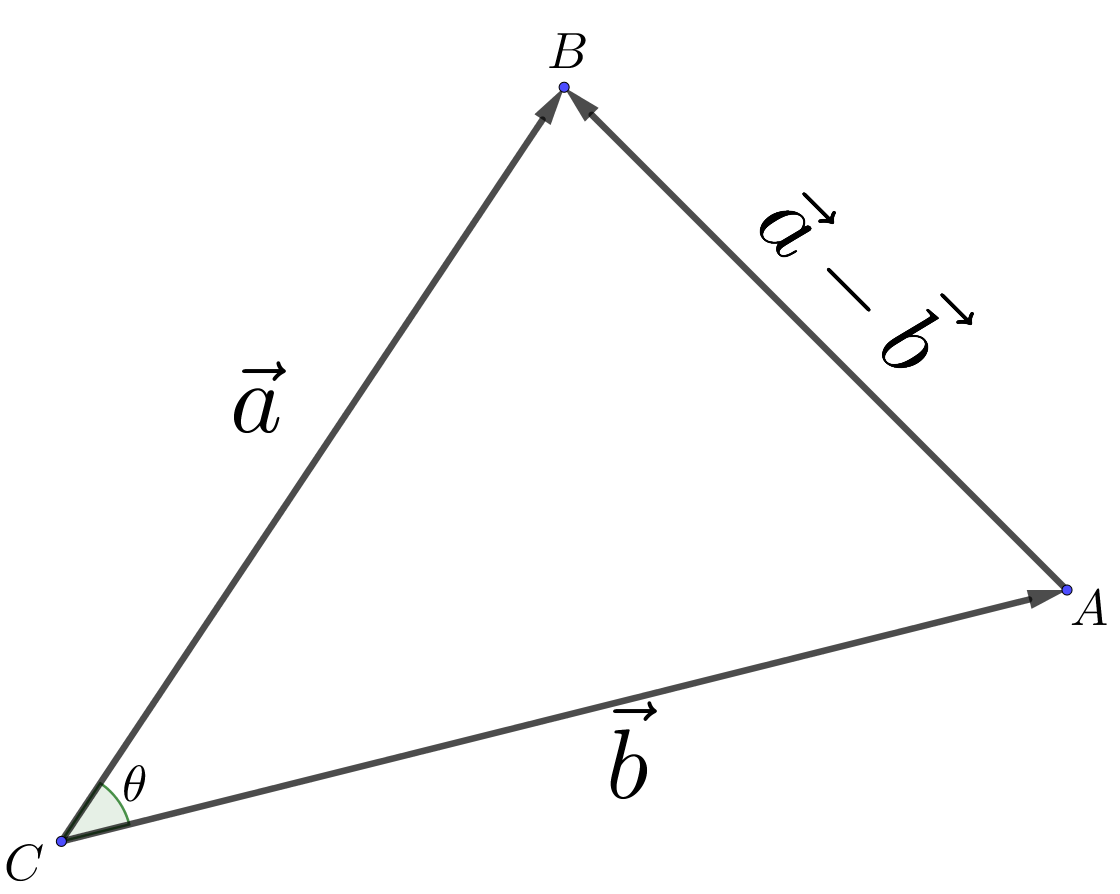
\includegraphics[scale=1.2]{angleBetweenVectors.png}
                \end{figure}
                
                Al aplicar ley de cosenos, tenemos que:
                \begin{align}
	                \Abs{\vec{a} - \vec{b}}^2 &= \Abs{\vec{a}}^2 + \Abs{\vec{b}}^2 - 2\Abs{\vec{a}}\Abs{\vec{b}}\cos\theta
                \end{align}
                
                Usamos la definición anterior para pasar de magnitud a producto punto:
                \begin{align}
	                \Wrap{\vec{a}-\vec{b}} \dotP \Wrap{\vec{a}-\vec{b}} &= \vec{a} \dotP \vec{a} + \vec{b} \dotP \vec{b} - 2\Abs{\vec{a}}\Abs{\vec{b}}\cos\theta
                \end{align}
                
                Ahora usamos la propiedad de linearidad dos veces y la conmutativa:
                \begin{align}
	                \vec{a} \dotP \Wrap{\vec{a}-\vec{b}} - \vec{b} \dotP \Wrap{\vec{a}-\vec{b}} &= \vec{a} \dotP \vec{a} + \vec{b} \dotP \vec{b} - 2\Abs{\vec{a}}\Abs{\vec{b}}\cos\theta\\
	                \vec{a} \dotP \vec{a} - 2\vec{a} \dotP \vec{b} + \vec{b} \dotP \vec{b} &= \vec{a} \dotP \vec{a} + \vec{b} \dotP \vec{b} - 2\Abs{\vec{a}}\Abs{\vec{b}}\cos\theta
                \end{align}
                
                Cancelamos términos comunes y simplificamos:
                \begin{align}
	                - 2\vec{a} \dotP \vec{b} = - 2\Abs{\vec{a}}\Abs{\vec{b}}\cos\theta\\
	                \boxed{\vec{a} \dotP \vec{b} = \Abs{\vec{a}}\Abs{\vec{b}}\cos\theta} \label{defDot2}
                \end{align}
                
                La ecuación (\ref{defDot2}) es una de las más importantes que involucran al producto punto, pues ahora lo relaciona con las magnitudes de los vectores y el ángulo entre ellos. A veces es común encontrar dicha ecuación como definición de producto punto y la que nosotros propusimos como consecuencia, ambas formas son correctas, pero creemos que es más fácil definirla de forma algebráica y luego deducir la forma geométrica.
                
                Ahora simplemente podemos despejar el coseno ángulo y obtenemos esta linda fórmula:
                \begin{align}
	                \cos \theta &= \dfrac{\vec{a} \dotP \vec{b}}{\Abs{\vec{a}} \Abs{\vec{b}}}
                \end{align}
                
                Como el rango de $\arccos$ va de $0$ a $\pi$, usando esta fórmula siempre obtendremos el ángulo correcto. Más aún, si $\theta=90^\circ$, entonces $\vec{a} \dotP \vec{b} = 0$. Esto nos motiva a definir lo siguiente, pues estos vectores recibirán un nombre especial:
                
                \begin{Definition}[Vectores ortogonales]
	                Sean $\vec{a}, \vec{b} \in \Reals^3$. Decimos que $\vec{a}$ y $\vec{b}$ son \textbf{ortogonales} si y solo si $\vec{a} \cdot \vec{b} = 0$.
                \end{Definition}
                
                % =========================================================
                % =============     PROYECCION DE VECTORES   ==============
                % =========================================================
                
                \clearpage
                \subsubsection{Proyección de un vector sobre otro}
                
                Ahora consideremos la siguiente situación:
                
                \begin{figure}[H]
                	\centering
                	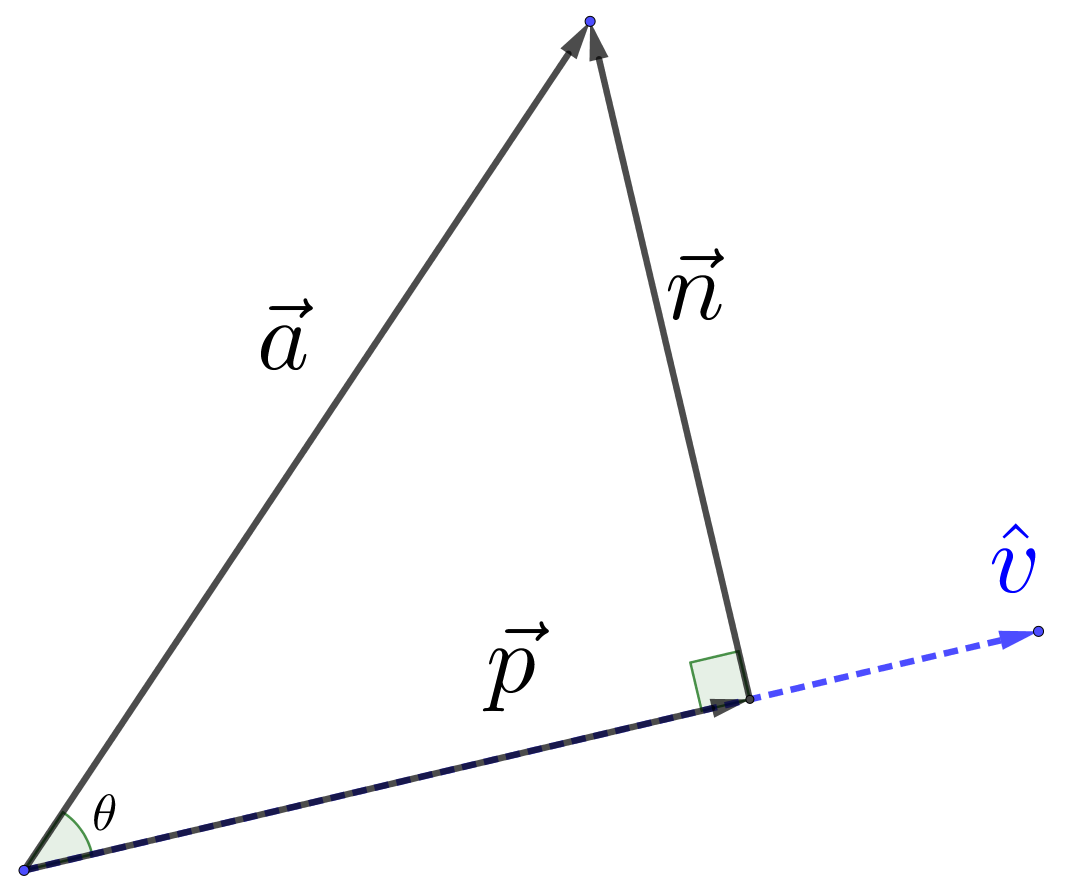
\includegraphics[scale=1.1]{vectorProyection.png}
                \end{figure}
            
            	Tenemos un vector cualquiera $\vec{a}$ y un vector unitario $\hat{v}$ que forman entre ellos un ángulo $\theta$. Queremos hallar la \emph{proyección} de $\vec{a}$ sobre la línea que genera la dirección de $\hat{v}$.
            	
            	Es decir, supongamos que extendemos el vector $\hat{v}$ para que forme un \Quote{piso}. Luego, colocamos al vector $\vec{a}$ en el mismo origen que $\hat{v}$, esta proyección nos dice la sombra que generaría $\vec{a}$ sobre el piso.
            	
            	Llamemos a la proyección $\vec{p}$, y al vector que resulta de unir la punta de $\vec{p}$ con la punta de $\vec{a}$ el vector $\vec{n}$ (al que llamaremos \emph{componente normal de $\vec{a}$ sobre $\hat{v}$}).
            	
            	Resulta claro que el ángulo que forma la punta de $\vec{p}$ con en inicio de $\vec{n}$ tiene que ser de $90^\circ$ por definición. De esa forma, aplicamos la definición del coseno para saber la magnitud de $\vec{p}$:
            	\begin{align}
	            	{\Abs{\vec{p}}} &= \Abs{\vec{a}} \cos \theta
            	\end{align}
            
            	Pero sabemos de la sección anterior que $\cos \theta = \dfrac{\vec{a} \dotP \hat{v}}{\Abs{\vec{a}} \Abs{\hat{v}}}=\dfrac{\vec{a} \dotP \hat{v}}{\Abs{\vec{a}}}$, entonces:
            	\begin{align}
	            	{\Abs{\vec{p}}} &= \cancel{\Abs{\vec{a}}} \dfrac{\vec{a} \dotP \hat{v}}{\cancel{\Abs{\vec{a}}}} = \vec{a} \dotP \hat{v}
            	\end{align}
                
                Ya tenemos la magnitud de $\vec{p}$, para determinarlo completamente solo nos hace falta su dirección, pero es claro que tiene que ser la misma de $\hat{v}$, y como $\hat{v}$ es unitario, simplemente multiplicamos:
                \begin{align}
	                \vec{p} = \Abs{\vec{p}} \hat{v} \implies \vec{p} = \Wrap{\vec{a} \dotP \hat{v}} \hat{v}
                \end{align}
                
                Finalmente, vemos de la figura que $\vec{p}+\vec{n}=\vec{a}$, entonces $\vec{n}=\vec{a}-\vec{p}$:
                \begin{align}
	                \vec{n} = \vec{a} - \Wrap{\vec{a} \dotP \hat{v}} \hat{v}
                \end{align}
                
                Los dos vectores anteriores son muy importantes que conviene \emph{definirlos}:
                
                % =========================================================
                % =================     DEFINICION   ======================
                % =========================================================
                
                \begin{Definition}[Proyección de vectores]
	                Sean $\vec{a}, \hat{v} \in \Reals^3$ con $\hat{v}$ unitario.
	                
	                Definimos a la \textbf{proyección de $\vec{a}$ sobre $\hat{v}$} como:
	                \begin{align}
		                proy_{\hat{v}}(\vec{a}) := \Wrap{\vec{a} \dotP \hat{v}} \hat{v} \label{defProj1}
	                \end{align}
	                
	                Y a la \textbf{componente normal de $\vec{a}$ sobre $\hat{v}$} como:
	                \begin{align}
	                \vec{n} := \vec{a} - \Wrap{\vec{a} \dotP \hat{v}} \hat{v} \label{defProj2}
	                \end{align}
                \end{Definition}
            
            	Si $\vec{v}$ no fuera unitario, simplemente lo normalizamos, además de que la fórmula se ve bonita asumiendo que es unitario. Si no lo fuera, tendríamos que $proy_{\vec{v}}(\vec{a}) := \dfrac{\Wrap{\vec{a} \dotP \vec{v}}\vec{v}}{\Abs{\vec{v}}^2}$.
            	
            	% =========================================================
            	% ==============     COSENOS DIRECTORES   =================
            	% =========================================================
                
                \subsubsection{Cosenos directores}
                
                Esta es una sección sencilla, se refiere a que dado un vector $\vec{a}=(a_1, a_2, a_3)$, lo proyectemos sobre los tres ejes $\mathbf{x}$, $\mathbf{y}$, $\mathbf{z}$ y obtengamos los tres ángulos.
                
                Para proyectarlo sobre el eje $\mathbf{x}$, tenemos que proyectar $\vec{a}$ sobre el vector unitario $\hat{i}$. Nombremos $\alpha$ al ángulo que forman, entonces:
                \begin{align}
	                \cos \alpha &= \dfrac{\vec{a} \dotP \hat{i}}{\Abs{\vec{a}} \Abs{\hat{i}}} = \dfrac{a_1}{\Abs{\vec{a}}}
                \end{align}
                
                Hacemos lo mismo con los otros ejes (el ángulo $\beta$ para el eje $\mathbf{y}$, $\gamma$ para el eje $\mathbf{z}$) y obtenemos:
                \begin{align}
	                \cos \beta &= \dfrac{a_2}{\Abs{\vec{a}}} \\
	                \cos \gamma &= \dfrac{a_3}{\Abs{\vec{a}}}
                \end{align}
                
                De esta forma, podemos escribir al vector unitario de $\vec{a}$ como $\hat{a} = (\cos \alpha)\hat{i}+(\cos \beta)\hat{j}+(\cos \gamma)\hat{k}$. Se queda como ejercicio que demuestres que $\hat{a}$ es realmente unitario.
                
                % =========================================================
                % ================     CAUCHY-SCHWARZ   ===================
                % =========================================================
                
                \subsubsection{Desigualdad de Cauchy-Schwarz}
                
                Esta es una de las desigualdades más poderosas, tanto que es muy usada en álgebra lineal.
                
                \begin{Theorem}[Desigualdad de Cauchy-Schwarz]
	                Sean $\vec{a}, \vec{b} \in \Reals^3$. Entonces:
	                \begin{align}
		                \abs{\vec{a} \dotP \vec{b}} \leq \Abs{\vec{a}} \Abs{\vec{b}} \label{CS-Inequality}
	                \end{align}
                \end{Theorem}
            
            	Es decir, el valor absoluto del producto punto de dos vectores siempre será menor o igual al producto de sus magnitudes.
            	
            	\begin{SmallIndentation}[1em]
            		\textbf{Demostración:} en este librito es suficiente con demostrarla para el espacio $\Reals^3$. Aunque también es válida para cualquier tipo de vectores de cualquier espacio vectorial con un producto interno.
            		
            		Supongamos que ningún vector es el cero vector. Si alguno lo fuera su magnitud sería cero y la desigualdad de Cauchy-Schwarz se cumple trivialmente.
            		
            		Sea $\theta$ el ángulo que forman $\vec{a}$ y $\vec{b}$. De trigonometría sabemos que $-1 \leq \cos \theta \leq 1$, entonces $\abs{\cos \theta} \leq 1$. Pero anteriormente deducimos que $\cos \theta = \dfrac{\vec{a} \cdot \vec{b}}{\Abs{\vec{a}} \Abs{\vec{b}}}$, entonces $\abs{\dfrac{\vec{a} \cdot \vec{b}}{\Abs{\vec{a}} \Abs{\vec{b}}}} \leq 1$, lo que implica que $\abs{\vec{a} \dotP \vec{b}} \leq \Abs{\vec{a}} \Abs{\vec{b}}$.
            	\end{SmallIndentation}
            
            	Una forma alternativa de esta desigualdad es usando la definición de valor absoluto (similar al coseno anteriormente): $-\Abs{\vec{a}} \Abs{\vec{b}} \leq \vec{a} \dotP \vec{b} \leq \Abs{\vec{a}} \Abs{\vec{b}}$.
                
                % =========================================================
                % ==========     DESIGUALDAD DEL TRIÁNGULO   ==============
                % =========================================================
                
                \clearpage
                
                \subsubsection{Desigualdad del triángulo}
                
                Es muy intuitiva de comprender, dice que la magnitud de la suma de dos vectores es menor o igual a la suma de sus magnitudes. Formalmente:
                
                \begin{Theorem}[Desigualdad del triángulo]
                	Sean $\vec{a}, \vec{b} \in \Reals^3$. Entonces:
                	\begin{align}
	                	\Abs{\vec{a}+\vec{b}} \leq \Abs{\vec{a}} + \Abs{\vec{b}} \label{triangleInequality}
                	\end{align}
                \end{Theorem}
            
            	Con dibujitos:
            	\begin{figure}[H]
            		\centering
            		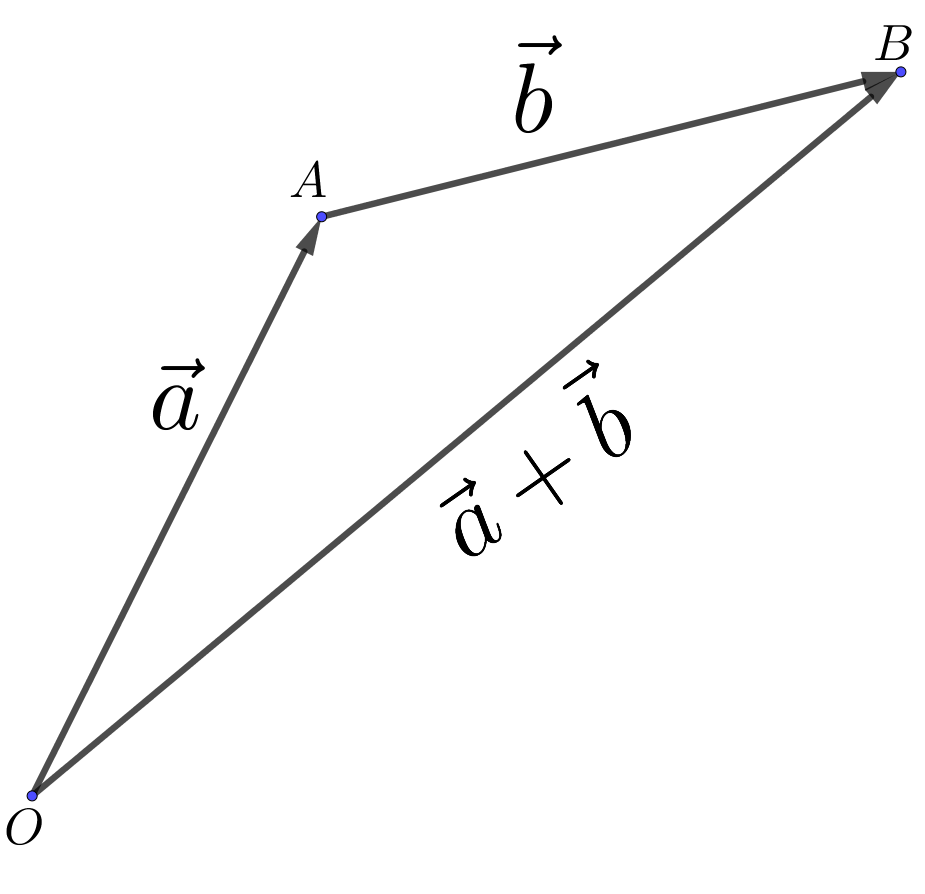
\includegraphics[scale=1]{triangleInequality.png}
            	\end{figure}
            
            	Vemos que la distancia más corta entre el origen $O$ y el punto $B$ tiene que ser un segmento de recta, justamente $\Abs{\vec{a}+\vec{b}}$. Si en vez de irnos directamente a $B$ nos vamos primero a $A$ y de ahí a $B$, habremos recorrido una mayor distancia, que es $\Abs{\vec{a}}+\Abs{\vec{b}}$. Pero claro, eso no es una demostración formal. Aquí viene la chida:
            	
            	% =========================================================
            	% =================     DEMOSTRACION   ====================
            	% =========================================================
            	
            	\begin{SmallIndentation}[1em]
            		\textbf{Demostración:} tratemos de usar todo lo aprendido hasta ahora, en especial el producto punto y la desigualdad de Cauchy-Schwarz. Comencemos del lado de $\Abs{\vec{a}+\vec{b}}$, pero elevado al cuadrado para poder pasar a producto punto sin que haya raíces:
            		\begin{align*}
	            		\Abs{\vec{a}+\vec{b}}^2 &= \Wrap{\vec{a}+\vec{b}} \dotP \Wrap{\vec{a}+\vec{b}} &&\mbox{Definición de magnitud}\\
	            		&= \vec{a} \dotP \vec{a} + 2\textcolor{blue}{\vec{a} \dotP \vec{b}} + \vec{b} \dotP \vec{b} &&\mbox{Propiedad distributiva}\\
	            		&\textcolor{blue}{\leq} \;\; \vec{a} \dotP \vec{a} + 2\textcolor{blue}{\Abs{\vec{a}}\Abs{\vec{b}}} + \vec{b} \dotP \vec{b} &&\textcolor{blue}{\mbox{Desigualdad de Cauchy-Schwarz}}\\
	            		&= \Abs{\vec{a}}^2 + 2\Abs{\vec{a}}\Abs{\vec{b}} + \Abs{\vec{b}}^2 &&\mbox{Definición de magnitud a la inversa}\\
	            		&= \Wrap{\Abs{\vec{a}} + \Abs{\vec{b}}}^2 &&\mbox{Factorizamos}
            		\end{align*}
            		
            		De esa forma obtenemos $\Abs{\vec{a}+\vec{b}}^2 \leq \Wrap{\Abs{\vec{a}} + \Abs{\vec{b}}}^2$. Como todas las magnitudes son no negativas, podemos sacar raíz cuadrada a ambos lados y concluir que $\Abs{\vec{a}+\vec{b}} \leq \Abs{\vec{a}} + \Abs{\vec{b}}$.
            	\end{SmallIndentation}
            
            \clearpage
            
            % =========================================================
            % =================     PRODUCTO CRUZ   ===================
            % =========================================================
            
            \subsection{Producto cruz}
            
            	Es el segundo tipo de producto que existe entre los vectores. Este sí es un producto \Quote{genuino} de vectores, porque el resultado ahora sí es otro vector. Sin embargo es un poco raro en comparación al producto punto, pues definirlo directamente de forma algebráica sería complicado y poco intuitivo. Además de que es obligatorio que trabajemos en $\Reals^3$ (porque está muy arraigado al espacio en 3D), pues en $\Reals^2$ no tiene sentido y en dimensiones superiores es bastante complicado generalizarlo.
            	
            	Dicho lo anterior, tratemos de definirlo primero de forma geométrica:
            	
            	% =========================================================
            	% ===================     DEFINICION   ====================
            	% =========================================================
            	
            	\begin{Definition}[Producto cruz]
	            	Sean $\vec{a}, \vec{b} \in \Reals^3$. Definimos al \textbf{producto cruz} o \textbf{producto vectorial} de $\vec{a}$ con $\vec{b}$ como:
	            	\begin{align}
		            	\vec{c} &= \vec{a} \times \vec{b} \label{defCross}
	            	\end{align}
	            	Donde: \begin{itemize}\setlength\itemsep{0em}
	            		\item $\Abs{\vec{c}}$ es el área del paralelogramo formado por los vectores $\vec{a}$ y $\vec{b}$:
	            		\begin{figure}[H]
	            			\centering
	            			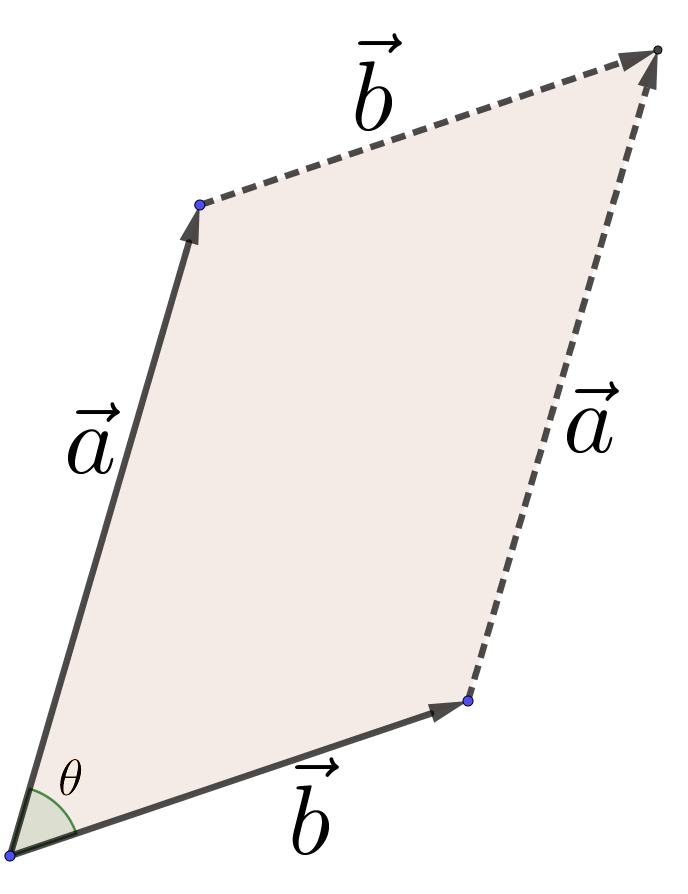
\includegraphics[scale=1.2]{parallelogram.png}
	            		\end{figure}
            			De geometría y trigonometría sabemos que dicha área es $\Abs{\vec{c}}=\Abs{\vec{a}} \Abs{\vec{b}} \sen \theta$, donde $0 \leq \theta \leq \pi$.
            			
            			\item La dirección de $\vec{c}$, es decir, $\hat{c}$, es perpendicular tanto a $\vec{a}$ como a $\vec{b}$, y de forma arbitraria vamos a proponer que se siga la famosa \textbf{regla de la mano derecha}, porque justamente en tu mano derecha el índice lo apuntas en dirección de $\vec{a}$ y el dedo medio en dirección de $\vec{b}$, tu pulgar apuntará en la dirección de $\hat{c}$.
            			\begin{figure}[H]
            				\centering
            				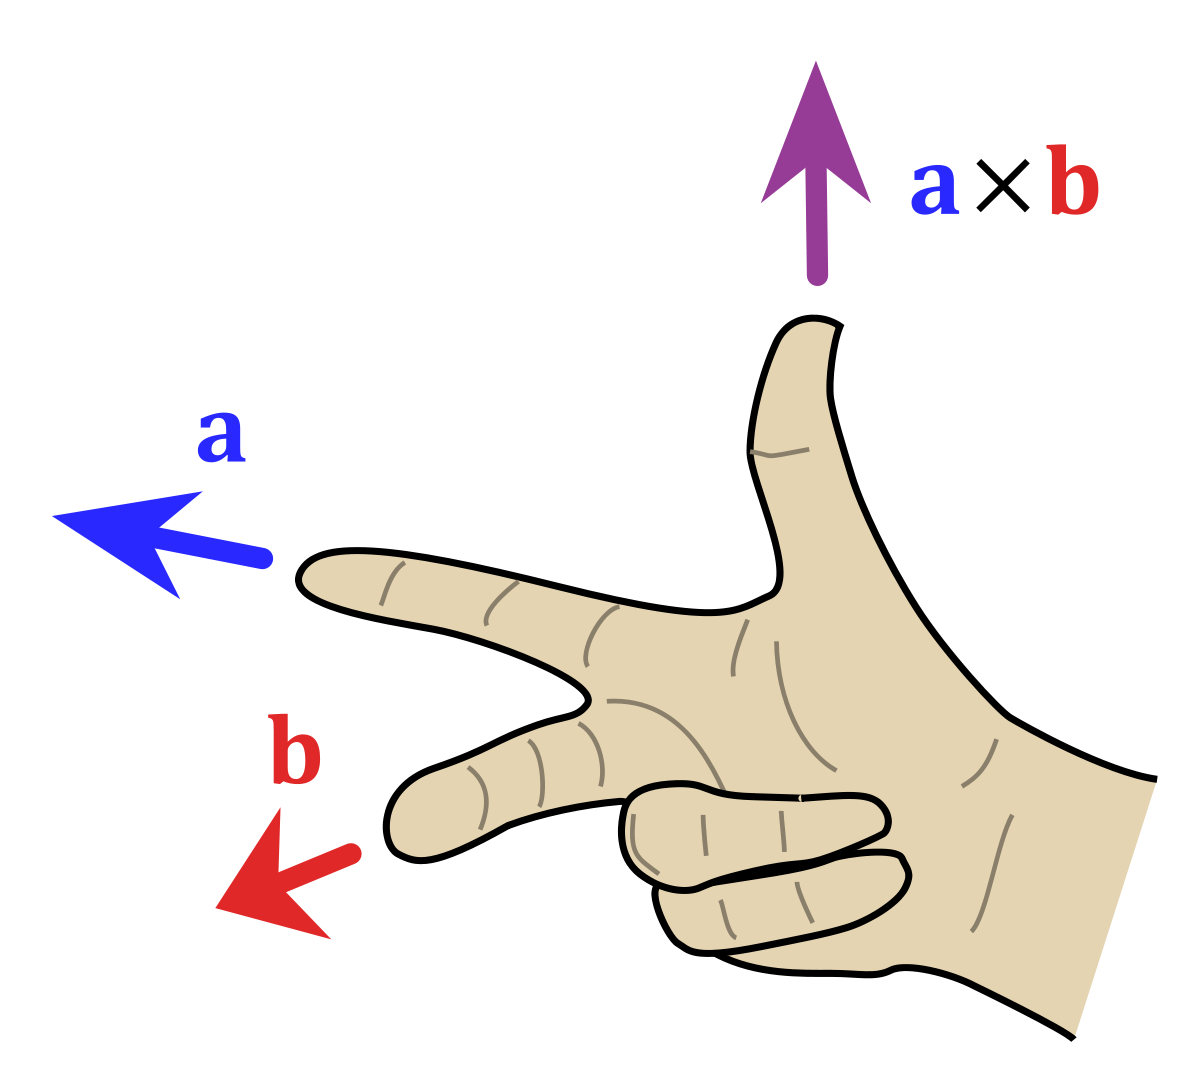
\includegraphics[scale=0.2]{rightHandRule.png}
            			\end{figure}
	            	\end{itemize}
            	\end{Definition}
            
            	Para hacer que la definición anterior sea verdaderamente útil, calculemos los productos cruz de los vectores unitarios canónicos $\hat{i}, \hat{j}, \hat{k}$:
            	
            	Si dibujamos los vectores $\hat{i}$ y $\hat{j}$, vemos que el paralelogramo que forman es justamente un cuadrado de área 1, pues el lado mide 1:
            	\begin{figure}[H]
            		\centering
            		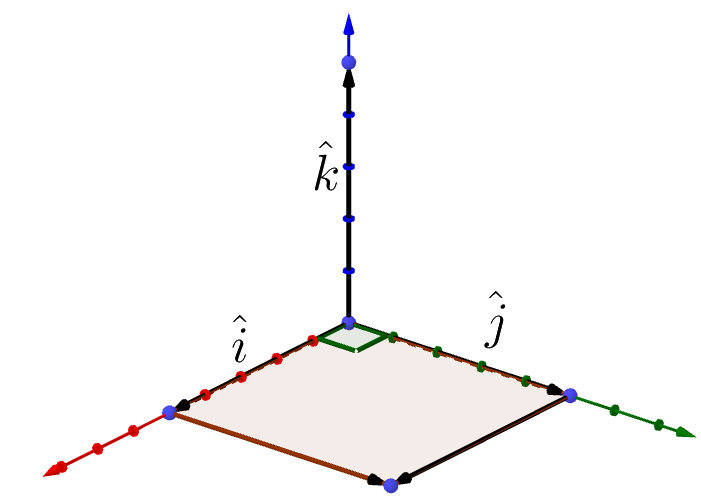
\includegraphics[scale=0.6]{unitVectors.png}
            	\end{figure}
            
            	De esta forma, $\Abs{\hat{i} \times \hat{j}} = 1$. También vemos que cualquier dirección perpendicular a $\hat{i}$ y a $\hat{j}$ simultáneamente tiene que apuntar a fuerzas hacia $\pm \hat{k}$. Pero por la regla de la mano derecha, nos quedamos con la positiva. Por lo tanto: $\hat{i} \times \hat{j} = \hat{k}$. De forma similar tomando los otros posibles pares de vectores unitarios canónicos, obtenemos las siguientes relaciones:
            	\begin{align}
	            	\hat{i} \times \hat{j} = \hat{k} \MegaSpace , \MegaSpace \hat{j} \times \hat{k} = \hat{i} \MegaSpace , \MegaSpace \hat{k} \times \hat{i} = \hat{j}
            	\end{align}
            	
            	Y también tenemos que:
            	\begin{align}
            		\hat{j} \times \hat{i} = -\hat{k} \MegaSpace &, \MegaSpace \hat{k} \times \hat{j} = -\hat{i} \MegaSpace &, \MegaSpace \hat{i} \times \hat{k} = -\hat{j}\\
            		\hat{i} \times \hat{i} = \vec{0} \MegaSpace &, \MegaSpace \hat{j} \times \hat{j} = \vec{0} \MegaSpace &, \MegaSpace \hat{k} \times \hat{k} = \vec{0}
            	\end{align}
            	
            	Ahora veamos algunas propiedades básicas del producto cruz para poder deducir una fórmula en términos de las componentes de los vectores:
            	
            	% =========================================================
            	% =================     PROPIEDADES   =====================
            	% =========================================================
            	
            	\begin{Theorem}
            		Tenemos las siguientes propiedades, donde $\vec{a}, \vec{b}, \vec{c} \in \Reals^3$ y $k \in \Reals$:
            		\begin{itemize}\setlength\itemsep{0em}
            			\item \textbf{Anticonmutatividad:} $\vec{a} \times \vec{b} = -\vec{b} \times \vec{a}$.
            			
            			\item \textbf{Distributiva por la izquierda:} $\vec{a} \times \Wrap{\vec{b}+\vec{c}} = \vec{a} \times \vec{b} + \vec{a} \times \vec{c}$.
            			
            			\item \textbf{Distributiva por la derecha:} $\Wrap{\vec{a}+\vec{b}} \times \vec{c} = \vec{a} \times \vec{c} + \vec{b} \times \vec{c}$.
            			
            			\item $k\Wrap{\vec{a} \times \vec{b}} = \Wrap{k \vec{a}} \times \vec{b} = \vec{a} \times \Wrap{k \vec{b}}$.
            			
            			\item $\vec{a} \times \vec{a} = \vec{0}$
            		\end{itemize}
            	\end{Theorem}
            
            	% =========================================================
            	% =================     DEMOSTRACION   ====================
            	% =========================================================
            
            	\begin{SmallIndentation}[1em]
            		\textbf{Demostración:}
            		\begin{itemize}\setlength\itemsep{0em}
            			\item Por definición, $\Abs{\vec{a} \times \vec{b}} = \Abs{\vec{a}} \Abs{\vec{b}} \sen \theta$. Como $\theta$ es en ángulo tanto \emph{entre $\vec{a}$ y $\vec{b}$} como \emph{entre $\vec{b}$ y $\vec{a}$}, entonces $\Abs{\vec{a} \times \vec{b}} = \Abs{\vec{b} \times \vec{a}}$.
            			
            			Ahora, usando regla de la mano derecha, si el dedo índice apunta en dirección de $\hat{a}$ y el medio en dirección de $\hat{b}$, el pulgar apuntará en dirección de $\vec{a} \times \vec{b}$. Por lo que si ahora el dedo índice apunta en dirección de $\hat{b}$ y el medio en dirección de $\hat{a}$, es obvio que el pulgar apuntará en dirección contraria a la que apuntaba antes.
            			
            			Concluyendo, $\vec{a} \times \vec{b} = -\vec{b} \times \vec{a}$.
            			
            			\item Pendiente.
            			
            			\item Misma idea que el inciso anterior.
            			
            			\item Veamos que $\Wrap{k \vec{a}} \times \vec{b} = k\Wrap{\vec{a} \times \vec{b}}$. Si $k=0$, ambos lados de la ecuación son el cero vector. En caso contrario, sea $\theta$ el ángulo entre $\vec{a}$ y $\vec{b}$.
            			
            			Si $k>0$, la dirección de $\Wrap{k \vec{a}} \times \vec{b}$ es la misma que la de $\vec{a} \times \vec{b}$ y la de $k\Wrap{\vec{a} \times \vec{b}}$. El ángulo entre $k\vec{a}$ y $\vec{b}$ también es el mismo que entre $\vec{a}$ y $\vec{b}$. Entonces:
            			\begin{align*}
	            			\Abs{(k\vec{a}) \times \vec{b}} &= \Abs{k\vec{a}} \Abs{\vec{b}} \sen \theta &&\mbox{Definición de producto cruz}\\
	            			&= k \Abs{\vec{a}} \Abs{\vec{b}} \sen \theta &&\mbox{Propiedad de la magnitud}\\
	            			&= k \Abs{\vec{a} \times \vec{b}} &&\mbox{Definición de producto cruz}\\
	            			&= \Abs{k\Wrap{\vec{a} \times \vec{b}}} && \mbox{Propiedad de la magnitud}
            			\end{align*}
            			Por lo tanto, en este caso $\Wrap{k\vec{a}} \times \vec{b} = k\Wrap{\vec{a} \times \vec{b}}$.
            			
            			Si $k<0$, la dirección de $\Wrap{k\vec{a}} \times \vec{b}$ es igual que la de $\Wrap{-\vec{a}} \times \vec{b}$ y que la de $-\Wrap{\vec{a} \times \vec{b}}$, por ello es la misma que la de $k\Wrap{\vec{a} \times \vec{b}}$. Entonces el ángulo entre $k\vec{a}$ y $\vec{b}$ es el suplementario del que existe entre $\vec{a}$ y $\vec{b}$, es decir, $\pi-\theta$. Por lo tanto:
            			\begin{align*}
	            			\Abs{(k\vec{a}) \times \vec{b}} &= \Abs{k\vec{a}} \Abs{\vec{b}} \sen(\pi-\theta) &&\mbox{Definición de producto cruz}\\
	            			&= \abs{k} \Abs{\vec{a}} \Abs{\vec{b}} \sen(\pi-\theta) &&\mbox{Propiedad de la magnitud}\\
	            			&= \abs{k} \Abs{\vec{a}} \Abs{\vec{b}} \sen \theta &&\mbox{Identidad trigonométrica}\\
	            			&= \abs{k} \Abs{\vec{a} \times \vec{b}} && \mbox{Definición de producto cruz}\\
	            			&= \Abs{k\Wrap{\vec{a} \times \vec{b}}} && \mbox{Propiedad de la magnitud}
            			\end{align*}
            			Por lo tanto, también en este caso $\Wrap{k\vec{a}} \times \vec{b} = k\Wrap{\vec{a} \times \vec{b}}$.
            			
            			Se queda como ejercicio ver que $k\Wrap{\vec{a} \times \vec{b}} = \vec{a} \times \Wrap{k \vec{b}}$.
            		\end{itemize}
            	\end{SmallIndentation}
            
            	Hay que tener cuidado, porque por lo general el producto cruz \textbf{no es asociativo}, es decir, $\vec{a} \times \Wrap{\vec{b} \times \vec{c}} \neq \Wrap{\vec{a} \times \Vector{b}} \times \vec{c}$; por lo tanto, la expresión $\vec{a} \times \vec{b} \times \vec{c}$ es ambigua si no se especifica en qué orden se deben evaluar.
            	
            	Ya con eso podemos dar la definición algebráica del producto cruz (la presentaremos como un teorema):
            	
            	% =========================================================
            	% ===================     DEFINICION   ====================
            	% =========================================================
            	
            	\begin{Theorem}[Definición algebráica de producto cruz]
            		Sean $\vec{a}, \vec{b} \in \Reals^3$ dados por sus coordenadas: $\vec{a}=a_1\hat{i} + a_2\hat{j} + a_3\hat{k}$ y $\vec{b}=b_1\hat{i} + b_2\hat{j} + b_3\hat{k}$. Entonces:
            		\begin{align}
	            		\vec{a} \times \vec{b} &=
	            		\begin{vmatrix}
		            		\hat{i} & \hat{j} & \hat{k}\\
		            		a_1 & a_2 & a_3\\
		            		b_1 & b_2 & b_3
	            		\end{vmatrix}
	            		= \begin{vmatrix}
	            			a_2 & a_3\\
	            			b_2 & b_3
	            		\end{vmatrix}\hat{i} - 
	            		\begin{vmatrix}
		            		a_1 & a_3\\
		            		b_1 & b_3
	            		\end{vmatrix}\hat{j} + 
	            		\begin{vmatrix}
		            		a_1 & a_2\\
		            		b_1 & b_2
	            		\end{vmatrix}\hat{k}\\
	            		&= (a_2b_3-a_3b_2)\hat{i} + (a_3b_1-a_1b_3)\hat{j} + (a_1b_2-a_2b_1)\hat{k}
            		\end{align}
            	\end{Theorem}
            
            	% =========================================================
            	% ==================     DEMOSTRACION   ===================
            	% =========================================================
            	
            	\begin{SmallIndentation}
	            	\textbf{Demostración:} usando todas las propiedades anteriores, tenemos que (esto se pone intenso):
	            	\begin{align*}
		            	\vec{a} \times \vec{b} &= \Wrap{a_1\hat{i} + a_2\hat{j} + a_3\hat{k}} \times \Wrap{b_1\hat{i} + b_2\hat{j} + b_3\hat{k}}\\
		            	&= \textcolor{blue}{\Wrap{a_1\hat{i} + a_2\hat{j} + a_3\hat{k}} \times \Wrap{b_1\hat{i}}}
		            	+ \textcolor{red}{\Wrap{a_1\hat{i} + a_2\hat{j} + a_3\hat{k}} \times \Wrap{b_2\hat{j}}}
		            	+ \textcolor{brown}{\Wrap{a_1\hat{i} + a_2\hat{j} + a_3\hat{k}} \times \Wrap{b_3\hat{k}}}\\
		            	&= \textcolor{blue}{\cancel{a_1b_1\hat{i}\times\hat{i}} + a_2b_1\hat{j}\times\hat{i} + a_3b_1\hat{k}\times\hat{i}}
		            	+ \textcolor{red}{a_1b_2\hat{i}\times\hat{j} + \cancel{a_2b_2\hat{j}\times\hat{j}} + a_3b_2\hat{k}\times\hat{j}}
		            	+ \textcolor{brown}{a_1b_3\hat{i}\times\hat{k} + a_2b_3\hat{j}\times\hat{k} + \cancel{a_3b_3\hat{k}\times\hat{k}}}\\
		            	&= -a_2b_1\hat{k} + a_3b_1\hat{j} + a_1b_2\hat{k} - a_3b_2\hat{i} - a_1b_3\hat{j} + a_2b_3\hat{i}\\
		            	&= (a_2b_3 - a_3b_2)\hat{i} - (a_1b_3 - a_3b_1)\hat{j} + (a_1b_2 - a_2b_1)\hat{k}\\
		            	&= \begin{vmatrix}
			            	a_2 & a_3\\
			            	b_2 & b_3
		            	\end{vmatrix}\hat{i} - 
		            	\begin{vmatrix}
			            	a_1 & a_3\\
			            	b_1 & b_3
		            	\end{vmatrix}\hat{j} + 
		            	\begin{vmatrix}
			            	a_1 & a_2\\
			            	b_1 & b_2
		            	\end{vmatrix}\hat{k}\\
		            	&= \begin{vmatrix}
			            	\hat{i} & \hat{j} & \hat{k}\\
			            	a_1 & a_2 & a_3\\
			            	b_1 & b_2 & b_3
		            	\end{vmatrix}
	            	\end{align*}
            	\end{SmallIndentation}
            
            	Lo ideal es simplemente memorizar la definición con el determinante, ya que las coordenadas de forma explícita no están muy sencillas. ¿Y ya viste por qué fue mejor comenzar con la definición geométrica? Haber definido al producto cruz por medio de sus coordenadas no hubiera sido nada intuitivo.
            	
            	Vemos también que el producto cruz nos permite calcular el ángulo entre vectores, pues:
            	\begin{align}
	            	\sen \theta &= \dfrac{\Abs{\vec{a} \times \vec{b}}}{\Abs{\vec{a}} \Abs{\vec{b}}}
            	\end{align}
            	
            	Sin embargo, puede que no obtengamos el ángulo correcto, porque el rango de $\arcsen$ cuando su argumento es positivo es de $0$ a $\frac{\pi}{2}$. Por eso es un poco más conveniente usar el producto punto para esto.
            	
            	Aunque podemos decir que $\vec{a} \times \vec{b} = \vec{0}$ si y solo si $\vec{a}$ es paralelo a $\Vector{b}$, es decir, forman un ángulo de $0^\circ$.
            
 	            \clearpage
            
                \subsubsection{Área de un triángulo}
                
                Si tenemos un triángulo con vértices $A$, $B$ y $C$, podemos calcular su área de una forma muy sencilla usando el producto cruz.
                
                Escogemos de forma arbitraria un vértice y calculamos los dos vectores de desplazamiento a los otros dos puntos. El área simplemente será la mitad de la magnitud del producto punto entre estos dos vectores, pues dos triángulos forman un paralelogramo.
                
                \begin{figure}[H]
                	\centering
                	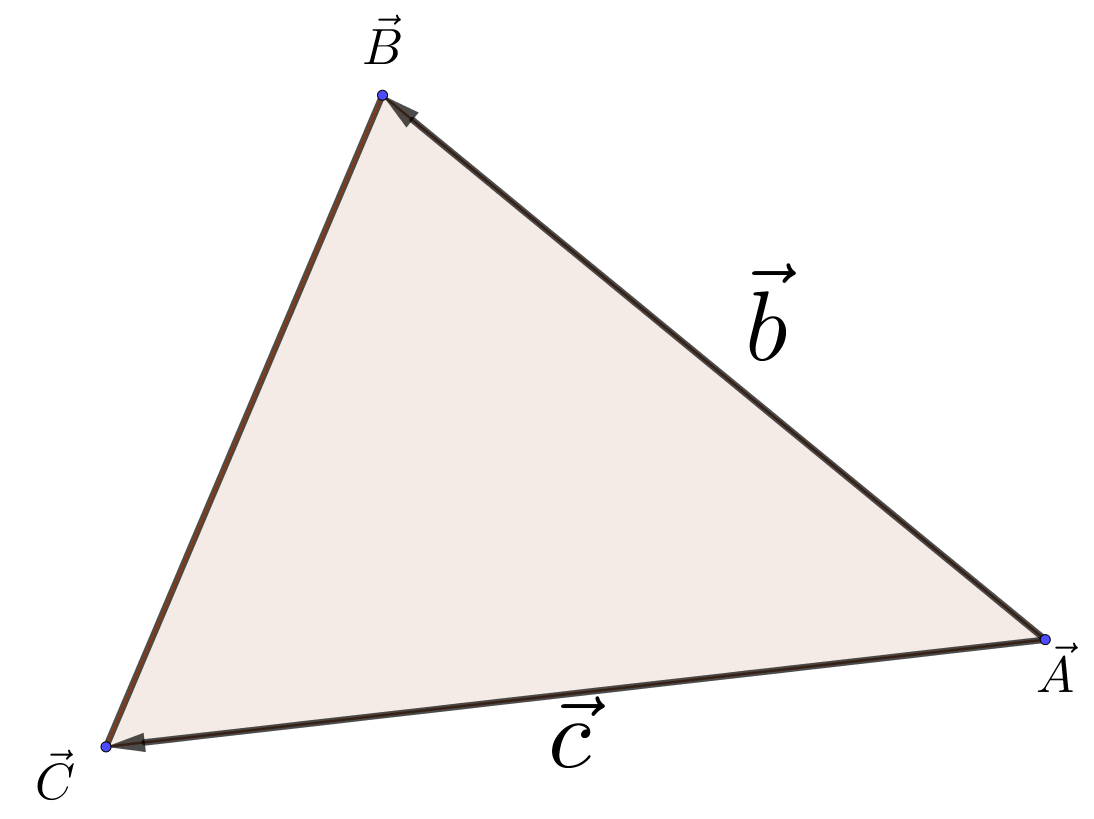
\includegraphics[scale=1.3]{triangle.png}
                \end{figure}
                
                Por ejemplo: supongamos que los vectores de posición del triángulo son $\vec{A}$, $\vec{B}$ y $\vec{C}$. Escogemos como referencia el vértice $\vec{A}$, de esta forma los vectores de desplazamiento son $\vec{b}=\vec{B}-\vec{A}$ y $\vec{c}=\vec{C}-\vec{A}$. Entonces el área será igual a $\dfrac{1}{2}\Abs{\vec{b} \times \vec{c}}$.
                
                \clearpage
                
                \subsubsection{Área de un paralelogramo en términos de sus diagonales}
                
                Sean $\vec{a}, \vec{b} \in \Reals^3$. Queremos hallar el área del paparelogramo que forman, pero no en términos de ellos, sino de las dos diagonales.
                
                \begin{figure}[H]
                	\centering
                	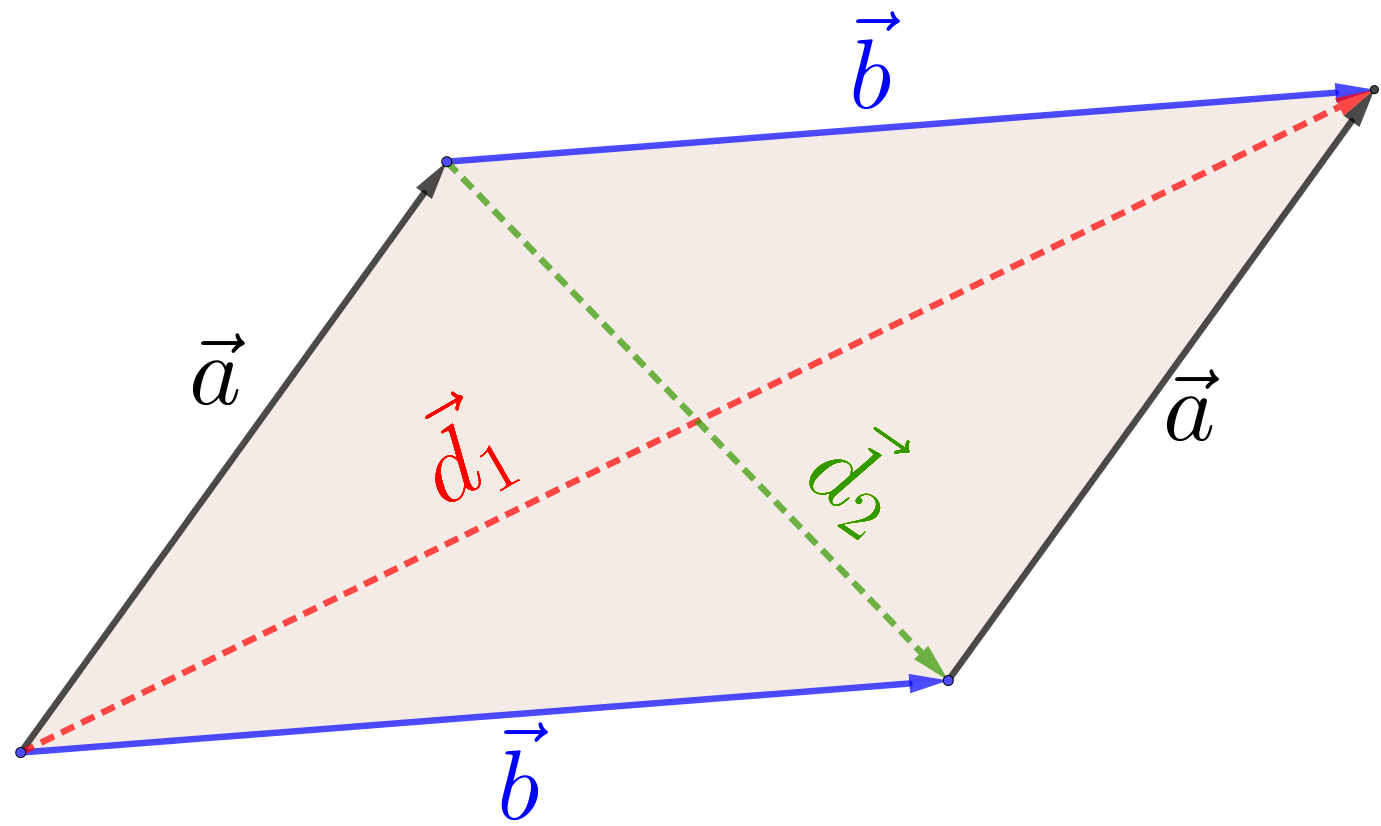
\includegraphics[scale=1.3]{parallelogram2.png}
                \end{figure}
            	
            	De la figura vemos que $\vec{d_1}=\vec{a}+\vec{b}$ y que $\vec{d_2}=\vec{b}-\vec{a}$, entonces hallemos $\vec{a}$ y $\vec{b}$ en términos de $\vec{d_1}$ y $\vec{d_2}$:
            	\begin{align*}
	            	\vec{a} &= \dfrac{1}{2}\Wrap{\vec{d_1}-\vec{d_2}}\\
	            	\vec{b} &= \dfrac{1}{2}\Wrap{\vec{d_1}+\vec{d_2}}
            	\end{align*}
            	
            	Por lo tanto, el área es:
            	\begin{align*}
	            	\Abs{\vec{a} \times \vec{b}} &= \Abs{\Wrap{\dfrac{1}{2}\Wrap{\vec{d_1}-\vec{d_2}}} \times \Wrap{\dfrac{1}{2}\Wrap{\vec{d_1}+\vec{d_2}}}} = \dfrac{1}{4} \Abs{\Wrap{\vec{d_1}-\vec{d_2}} \times \Wrap{\vec{d_1}+\vec{d_2}}}\\
	            	&= \dfrac{1}{4}\Abs{\cancel{\vec{d_1} \times \vec{d_1}} + \vec{d_1} \times \vec{d_2} - \vec{d_2} \times \vec{d_1} - \cancel{\vec{d_2} \times \vec{d_2}}}\\
	            	&= \dfrac{1}{4}\Abs{\vec{d_1} \times \vec{d_2} + \vec{d_1} \times \vec{d_2}}\\
	            	&= \dfrac{1}{4}\Abs{2\Wrap{\vec{d_1} \times \vec{d_2}}}\\
	            	&= \dfrac{1}{2}\Abs{\vec{d_1} \times \vec{d_2}}
            	\end{align*}
            	
            % =========================================================
            % =================     PRODUCTO TRIPLE   =================
            % =========================================================
            
            \subsection{Producto triple}
            
            	Este no es un nuevo producto, sino más bien una combinación de los dos anteriores.
            	
            	\begin{Definition}[Producto triple escalar]
	            	Sean $\vec{a}, \vec{b}, \vec{c} \in \Reals^3$. Definimos al \textbf{producto triple escalar} como $\vec{a} \dotP \Wrap{\vec{b} \times \vec{c}}$. Nota que de nuevo el resultado es un escalar y no un vector. También se suele usar la notación $\Brackets{\vec{a}, \vec{b}, \vec{c}} = \vec{a} \dotP \Wrap{\vec{b} \times \vec{c}}$.
            	\end{Definition}
            
            	Tenemos la siguiente propiedad:
            	
            	\begin{Theorem}[Permutación circular]
            		$\vec{a} \dotP \Wrap{\vec{b} \times \vec{c}} = \vec{b} \dotP \Wrap{\vec{c} \times \vec{a}} = \vec{c} \dotP \Wrap{\vec{a} \times \vec{b}}$
            	\end{Theorem}
            
            	\begin{SmallIndentation}[1em]
            		\textbf{Demostración:} vemos que los vectores $\vec{a}+\vec{b}$ y $\Wrap{\vec{a}+\vec{b}} \times \vec{c}$ son perpendiculares por definición. Es decir, forman un ángulo de $90^\circ$. Por lo tanto:
            		\begin{align*}
	            		\Wrap{\vec{a}+\vec{b}} \dotP \Wrap{\Wrap{\vec{a}+\vec{b}} \times \vec{c}} &= 0 &&\mbox{Los vectores son ortogonales}\\
	            		\Wrap{\vec{a}+\vec{b}} \dotP \Wrap{\vec{a} \times \vec{c} + \vec{b} \times \vec{c}} &= 0 &&\mbox{Propiedad distributiva}\\
	            		\cancel{\vec{a} \dotP \Wrap{\vec{a} \times \vec{c}}} + \vec{a} \dotP \Wrap{\vec{b} \times \vec{c}} + \vec{b} \dotP \Wrap{\vec{a} \times \vec{c}} + \cancel{\vec{b} \dotP \Wrap{\vec{b} \times \vec{c}}} &= 0 &&\mbox{Propiedad distributiva}\\
	            		\vec{a} \dotP \Wrap{\vec{b} \times \vec{c}} &= -\vec{b} \dotP \Wrap{\vec{a} \times \vec{c}} &&\mbox{Reacomodamos}\\
	            		\vec{a} \dotP \Wrap{\vec{b} \times \vec{c}} &= \vec{b} \dotP \Wrap{\vec{c} \times \vec{a}} &&\mbox{Anticonmutatividad}
            		\end{align*}
            		La segunda parte de la igualdad se sigue inmediatamente, haciendo que $\vec{a} \to \vec{b}$, $\vec{b} \to \vec{c}$ y $\vec{c} \to \vec{a}$, por eso recibe el nombre de permutación circular, pues las variables se van permutando cíclicamente.
            	\end{SmallIndentation}
            
            	\clearpage
            
                \subsubsection{Volumen de un paralelepípedo}
            
            	Supongamos que queremos hallar el volumen del paralelepípedo formado por los vectores $\vec{a}, \vec{b}$ y $\vec{c}$:
            
            	\begin{figure}[H]
            		\centering
            		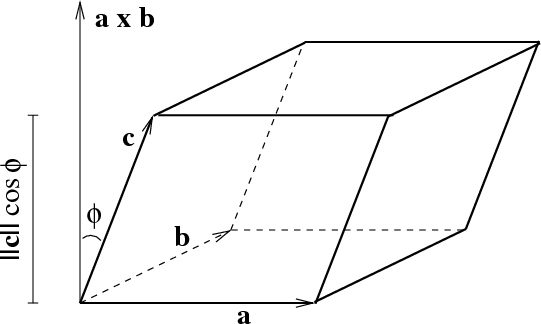
\includegraphics[scale=0.8]{parallelepiped.png}
            	\end{figure}
            
            	Recordemos que el volumen está dado por $V=\Wrap{\text{área de la base}}\Wrap{\text{altura}}$.
            	
            	Vemos que el área de la base es simplemente el área del paralelogramo formado por $\vec{a}$ y $\vec{b}$, es decir, $\Abs{\vec{a} \times \vec{b}}$.
            	
            	Sea $\phi$ el ángulo que forma el vector $\vec{a} \times \vec{b}$ con $\vec{c}$. Entonces, usando la definición de coseno vemos que la altura está dada por $\Abs{\vec{c}} \abs{\cos \phi}$. Usamos el valor absoluto en el coseno porque $\phi$ puede ser mayor a $90^\circ$, causando que $\cos \phi < 0$.
            	
            	De esa forma, el volumen es $V=\Abs{\vec{a} \times \vec{b}} \Abs{\vec{c}} \abs{\cos \phi}=\abs{\Abs{\vec{a} \times \vec{b}} \Abs{\vec{c}} \cos \phi}=\abs{\vec{c} \dotP \Wrap{\vec{a} \times \vec{b}}}$, que es justamente el valor absoluto del producto triple de los vectores que definen al paralelepípedo.
            	
            	¿Qué significado tendrá el hecho de que $\vec{a} \dotP \Wrap{\vec{b} \times \vec{c}}=0$? Quiere decir que el paralelepípedo no tiene volumen, es decir, que los tres vectores \textbf{están en el mismo plano}. Veremos más adelante las propiedades del plano.
            	
            	La expresión \emph{producto triple} puede hacer referencia a otras combinaciones donde estén involucrados tres vectores y sus productos, como $\vec{a} \times \Wrap{\vec{b} \times \vec{c}}$, $\Wrap{\vec{a} \dotP \vec{b}}\vec{c}$, etc.
            	
            	Antes de terminar con esta parte, veamos un último teorema:
            	
            	\begin{Theorem}
            		Sean $\vec{a}=a_1\hat{i}+a_2\hat{j}+a_3\hat{k}$, $\vec{b}=b_1\hat{i}+b_2\hat{j}+b_3\hat{k}$ y $\vec{c}=c_1\hat{i}+c_2\hat{j}+c_3\hat{k}$. Entonces:
            		\begin{align}
	            		\vec{a} \dotP \Wrap{\vec{b} \times \vec{c}} &= \begin{vmatrix}
		            		a_1 & a_2 & a_3\\
		            		b_1 & b_2 & b_3\\
		            		c_1 & c_2 & c_3
	            		\end{vmatrix}
            		\end{align}
            		Esto nos facilita mucho el cálculo del producto triple escalar, pues se reduce a que calculemos un determinante de dimensión 3, el cual es muy sencillo.
            	\end{Theorem}
            	
            	\begin{SmallIndentation}[1em]
            		\textbf{Idea de la demostración:} simplemente calcula ambos lados de la ecuación y comprueba que sean iguales. Es fácil pero tedioso.
            	\end{SmallIndentation}
            
            
            
            
    
    
    % ===============================================================================
    % ==============            APLICACIONES A LA GEOMETRIA         =================
    % ===============================================================================        
            
            
    \chapter{Aplicaciones a la geometría}
    
    	% =========================================================
    	% ====================     PLANOS   =======================
    	% =========================================================
        
        \section{Ecuación del plano}
        
        El plano es un objeto bidimensional que contiene infinitos puntos y rectas. Usualmente se les denota con la letra griega $\Pi$. Para definirlo, podemos contar con la siguiente información: \begin{itemize}\setlength\itemsep{0em}
	        \item Un punto por el que pasa y un vector normal a toda su superficie.
	        \item Tres puntos no colineales (que no estén en la misma recta) por los que pasa.
	        \item Un punto por el que pasa y dos vectores paralelos al plano.
        \end{itemize}
    
    	Aunque existen muchas más combinaciones que nos pueden determinar de forma única un plano.
    
    		% =========================================================
    		% =============     PUNTO Y VECTOR NORMAL   ===============
    		% =========================================================
    
    		\clearpage
    
    		\subsection{Punto y vector normal}
    		
    		Supongamos que el plano pasa por el punto $P$ y el vector normal a su superficie es $\vec{n}$. Queremos hallar un vector $\vec{r}$ tal que su flecha dibuje todo el plano.
    		
    		\begin{figure}[H]
    			\centering
    			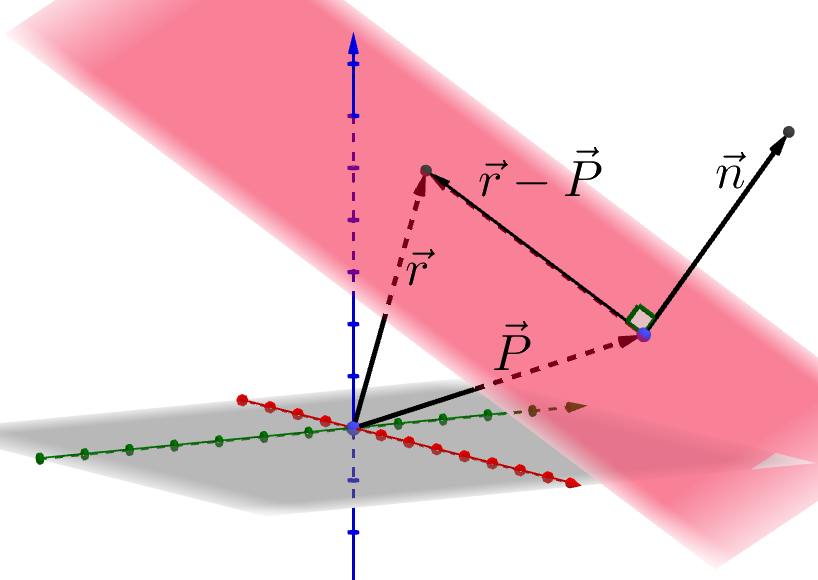
\includegraphics[scale=0.65]{plane.png}
    		\end{figure}
    		
    		De la figura vemos que $\vec{r} - \vec{P}$ siempre está contenido en el plano, y por ser así, será perpendicular a $\vec{n}$, por lo que:
    		\begin{align}
	    		\vec{n} \dotP \Wrap{\vec{r} - \vec{P}} &= 0 \label{planeEquationGeneral}
    		\end{align}
    		
    		Supongamos que $\vec{r}=(x,y,z)$, $\vec{n}=(a,b,c)$ y $\vec{P}=(x_0, y_0, z_0)$. Entonces podemos reescribir la ecuación:
    		\begin{align}
	    		&(a,b,c) \dotP \Wrap{x-x_0, y-y_0, z-z_0} = 0 \nonumber \\
	    		&\implies a(x-x_0) + b(y-y_0) + c(z-z_0) = 0 \\
	    		&\implies ax+by+cz = d \label{planeEquation1}
    		\end{align}
    		
    		Donde $d=ax_0 + by_0 + cz_0$. Como puedes ver, la ecuación del plano es muy sencilla en forma cartesiana, y podemos identificar rápidamente al vector normal con tan solo fijarnos en los coeficientes. Además ten en cuenta un mismo plano puede tener más de una ecuación que lo represente (infinitas de hecho), pues cualquier múltiplo escalar del vector normal es válido.
    		
    		% =========================================================
    		% =================     TRES PUNTOS   =====================
    		% =========================================================
    		
    		\subsection{Tres puntos}
    		
    		De forma similar a como calculábamos el área de un triángulo, vamos a escoger uno de los tres puntos y hallar los vectores de desplazamiento de él hacia los otros dos:
    		
    		\begin{figure}[H]
    			\centering
    			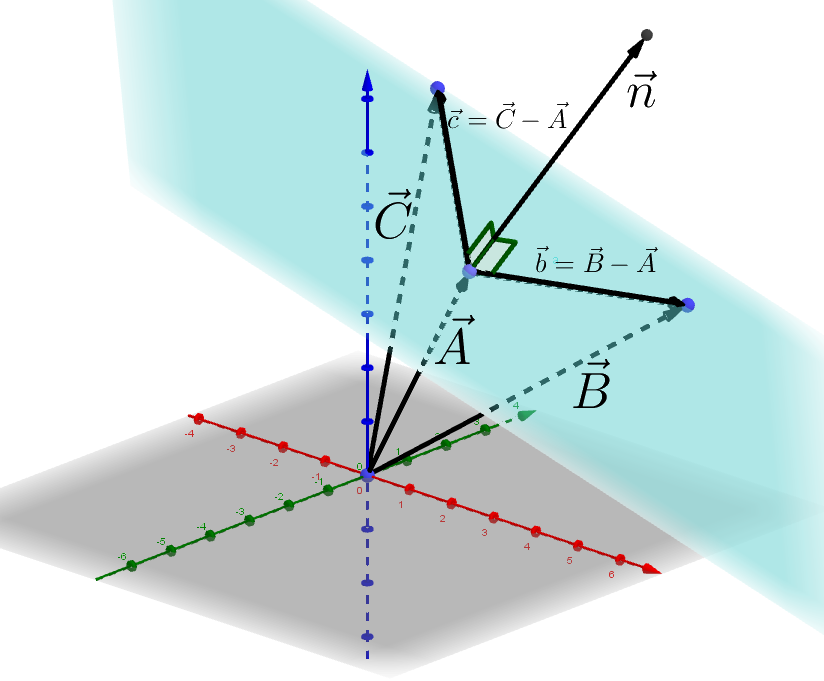
\includegraphics[scale=0.65]{plane2.png}
    		\end{figure}
    	
    		Por ejemplo, escojamos el punto $\vec{A}$ y a partir de ahí calculemos los vectores de desplazamiento $\vec{b}=\vec{B}-\vec{A}$ y $\vec{c}=\vec{C}-\vec{A}$. Vemos que tanto $\vec{b}$ como $\vec{c}$ están contenidos totalmente en el plano, lo que nos falta es hallar el vector normal, que debe ser perpendicular a ellos dos. Por definición del producto cruz, ese vector es simplemente $\vec{n}=\vec{b} \times \vec{c}$. Finalmente, escogemos cualquiera de los tres puntos y la ecuación del plano será:
    		\begin{align}
	    		&\vec{n} \dotP \Wrap{\vec{r} - \vec{A}} = 0 \nonumber \\
	    		&\implies \Wrap{\vec{b} \times \vec{c}} \dotP \Wrap{\vec{r} - \vec{A}} = 0 \label{planeEquation2}
    		\end{align}
    		
    		La forma difícil de calcular la ecuación del plano dados tres puntos, es sustituir cada uno en la ecuación general $ax+by+cz=d$ y formar un sistema de ecuaciones para hallar $a,b,c,d$. Sin embargo, es más tardado y al hacerlo así no entendemos realmente la geometría del problema.
    		
    		% =========================================================
    		% ========     PUNTO Y DOS VECTORES PARALELOS   ===========
    		% =========================================================
    		
    		\subsection{Punto y dos vectores paralelos}
    		
    		Similar a la situación anterior, solo que ahora nos dan un punto por el que pasa ($\vec{A}$) y los dos vectores paralelos, que ahora llamaremos $\lVec{e_1}$ y $\lVec{e_2}$. Veremos que podemos escribir la ecuación del plano de otra manera:
    		
    		\begin{figure}[H]
    			\centering
    			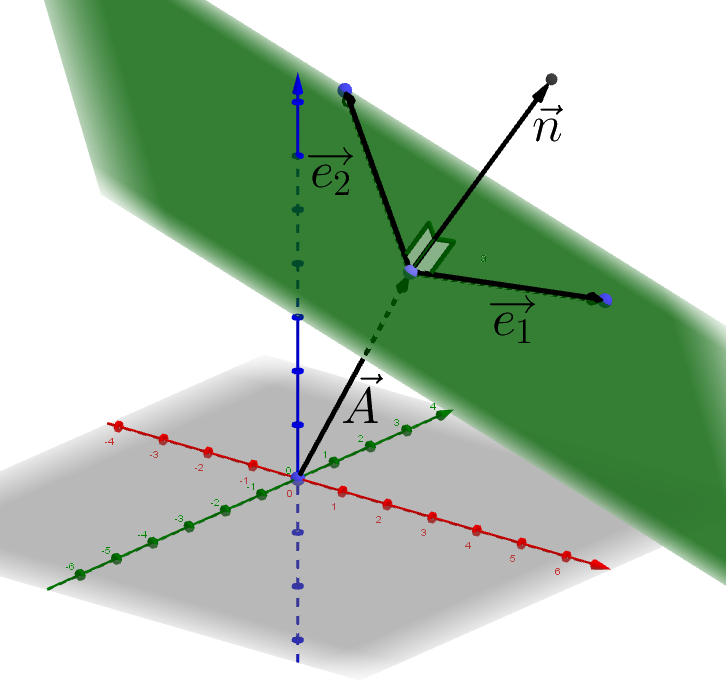
\includegraphics[scale=0.65]{plane3.png}
    		\end{figure}
    	
    		Como el plano tiene dos dimensiones, intuitivamente podemos decir que tenemos dos \Quote{grados de libertad} de movimiento, es decir, que podemos movernos lo que queramos en la dirección de $\lVec{e_1}$ y lo que queramos en la dirección de $\lVec{e_2}$. El efecto de \Quote{movernos} no es más que multiplicar a esos vectores por un escalar. Lo que significa que cualquier punto en el plano puede ser expresado como:
    		\begin{align}
	    		\vec{r} &= \vec{A} + s\lVec{e_1} + t\lVec{e_2} \label{planeEquation3}
    		\end{align}
    		
    		Donde $s, t \in \Reals$, es decir, abarcan todos los números reales para \Quote{barrer} todo el plano. Le sumamos el vector $\vec{A}$ para forzar que el plano pase por ahí. Esta forma de escribir la ecuación del plano se conoce como \emph{ecuación paramétrica}, que estudiaremos más adelante.
    		
    		\textbf{Nota:} es muy importante que $\lVec{e_1}$ y $\lVec{e_2}$ sean linealmente independientes para poder definir un plano. ¿Qué pasaría si fueran linealmente dependientes? Pista: uno sería múltiplo escalar del otro, así que...
    		
    	% =========================================================
    	% ====================     RECTAS   =======================
    	% =========================================================
    	
    	\clearpage
            
        \section{Ecuación de la recta}
        
        Una recta es el conjunto de puntos que se mueven en una dirección determinada, y de forma indefinida en sus ambos extremos. Existen dos formas principales de definirlas: \begin{itemize}\setlength\itemsep{0em}
        	\item Mediante un punto por el que pasa y un vector paralelo a ella.
        	\item Mediante dos puntos por los que pasa.
        \end{itemize}
    
    		% =========================================================
    		% ============     PUNTO Y VECTOR PARALELO   ==============
    		% =========================================================
    		
    		\clearpage
    
    		\subsection{Punto y vector paralelo}
    		
    		Supongamos que la recta pasa por el punto $P$ y un vector paralelo a ella es $\vec{v}$. Vemos que la tarea de $\vec{v}$ es básicamente darle la dirección a la recta:
    		
    		\begin{figure}[H]
    			\centering
    			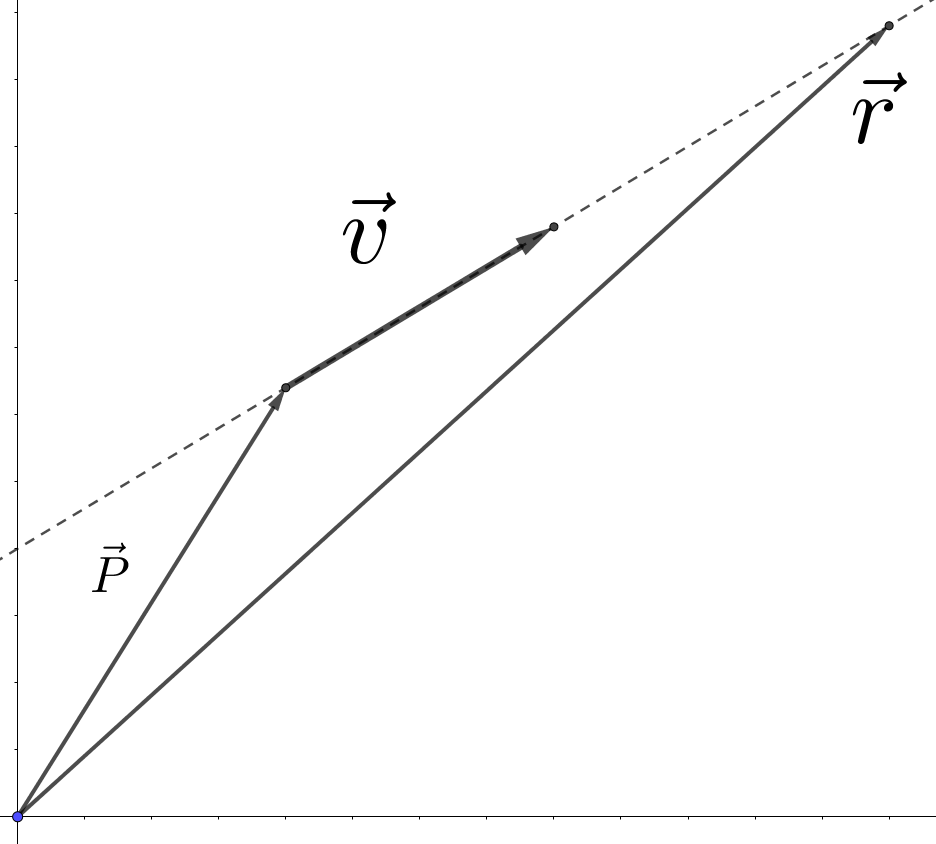
\includegraphics[scale=1.2]{line.png}
    		\end{figure}
        
        	Sea $\vec{r}$ el vector de posición de cada uno de los puntos de la línea, es decir, su flecha va a barrer a toda la línea. En este caso solo podemos movernos en la dirección de $\vec{v}$, por lo que cualquier múltiplo escalar de $\vec{v}$ estará sobre la línea, sumándole el punto $\vec{P}$. Entonces:
        	\begin{align}
	        	\vec{r} &= \vec{P} + t\vec{v} \label{lineEquationGeneral}
        	\end{align}
        	
        	Donde $t \in \Reals$. La ecuación anterior es conocida como la \emph{ecuación paramétrica de la recta}, de forma similar a la del plano. Si $\vec{r}=(x,y,z)$, $\vec{v}=(a,b,c)$ y $\vec{P}=(x_0,y_0,z_0)$, entonces podemos reescribirla como:
        	\begin{align*}
	        	(x, y, z) &= (x_0 + ta, y_0 + tb, z_0 + tc)
        	\end{align*}
        	
        	Comparamos componente a componente y despejamos $t$ en cada caso:
        	\begin{align*}
	        	x &= x_0 + ta &\implies t = \dfrac{x - x_0}{a} \\
	        	y &= y_0 + tb &\implies t = \dfrac{y - y_0}{b} \\
	        	z &= z_0 + tc &\implies t = \dfrac{z - z_0}{c}
        	\end{align*}
        	
        	Igualamos y obtenemos la forma cartesiana de la ecuación de la recta:
        	\begin{align}
	        	\dfrac{x - x_0}{a} = \dfrac{y - y_0}{b} = \dfrac{z - z_0}{c} \label{lineEquation1}
        	\end{align}
        	
        	Nota que una misma línea puede tener varias ecuaciones, pues cualquier múltiplo escalar de $\vec{v}$ funciona. Además, para usar la forma cartesiana requerimos que $a,b,c\neq 0$, mientras que en la forma paramétrica no hay restricción.
        	
        	% =========================================================
        	% ==================     DOS PUNTOS   =====================
        	% =========================================================
        	
        	\subsection{Dos puntos}
        	
        	Ahora supongamos que nos dan dos puntos $\vec{A}$ y $\vec{B}$, y queremos hallar la ecuación de la recta que pasa por ellos:
        	
        	\begin{figure}[H]
        		\centering
        		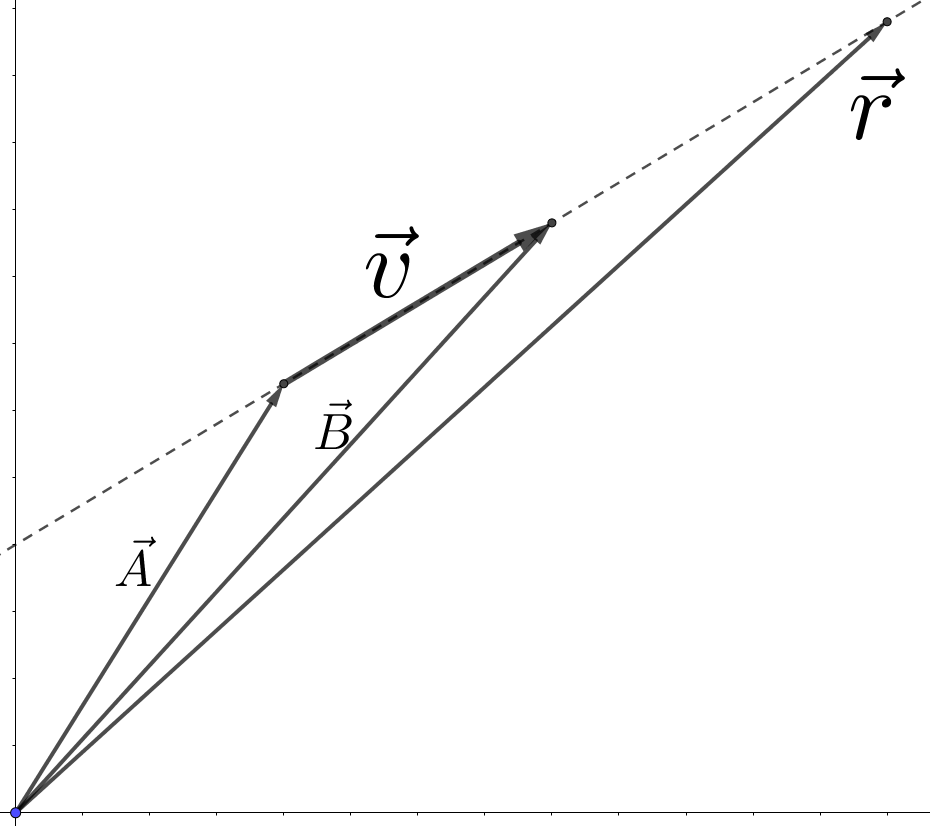
\includegraphics[scale=1.2]{line2.png}
        	\end{figure}
        
        	De la figura vemos que $\vec{A}+\vec{v}=\vec{B}$, entonces el vector paralelo es simplemente $\vec{v}=\vec{B}-\vec{A}$. Por lo tanto, la ecuación de la recta paramétrica queda como:
        	\begin{align}
	        	\vec{r} &= \vec{A} + t\Wrap{\vec{B}-\vec{A}} = (1-t)\vec{A}+t\vec{B} \label{lineEquation2}
        	\end{align}
        	
        	Nota que también podemos usar el punto $\vec{B}$ como punto inicial.
        	
        	Ahora, si $\vec{A}=(x_1, y_1, z_1)$ y $\vec{B}=(x_2, y_2, z_2)$, siguiendo una deducción similar a la de la sección anterior, la ecuación en forma cartesiana queda como:
        	\begin{align}
	        	\dfrac{x - x_1}{x_2 - x_1} = \dfrac{y - y_1}{y_2 - y_1} = \dfrac{z - z_1}{z_2 - z_1} \label{lineEquation3}
        	\end{align}
        	
        	Nota su parecido con la ecuación de la recta en dos dimensiones que probablemente conozcas de geometría analítica.
        
        \section{Ecuación de la esfera}
            
        \section{Distancia punto-recta y punto-plano}
        
        \section{Rotaciones en el espacio}
        
        \section{Demostraciones geométricas mediante vectores}
            


\part{Cálculo diferencial vectorial}

    \chapter{Funciones de varias variables}
    
        \section{Representación como superficies}
        
            \subsection{Curvas de nivel y de contorno}
            
        \section{Límites}
            
            \subsection{Definición intuitiva}
            
            \subsection{Definición formal}
            
        \section{Continuidad}
        
        \section{Derivadas parciales}
        
            \subsection{Plano tangente a una superficie}
            
            \subsection{Diferenciabilidad}
            
            \subsection{Derivadas de orden superior}
            
                \subsubsection{Teorema de Clairaut}
                
        \section{Gradiente}
                
        \section{Regla de la cadena}
        
            \subsection{Diferencial total}
            
        \section{Derivada direccional}
        
        \section{Puntos críticos}
        
            \subsection{Máximos, mínimos y puntos silla}
            
            \subsection{Criterio del hessiano}
            
        \section{Multiplicadores de Lagrange}


    \chapter{Funciones vectoriales}
    
        \section{Curvas en forma paramétrica}
        
            \subsection{Reglas de derivación}
            
            \subsection{Velocidad y aceleración}
        
            \subsection{Longitud de arco}
            
            \subsection{Parametrización por longitud de arco}
            
            \subsection{Geometría diferencial}
                
                \subsubsection{Vector tangente, normal y binormal}
                
                \subsubsection{Curvatura y torsión}
                
                \subsubsection{Velocidad y aceleración}
                
                \subsubsection{Ecuaciones de Frenet-Serret}
            
        \section{Campos vectoriales}
        
            \subsection{Líneas de campo}
            
            \subsection{Derivadas parciales}
        
        \section{Operador nabla}
        
            \subsection{Gradiente}
            
            \subsection{Divergencia}
            
            \subsection{Rotacional}
            
            \subsection{Laplaciano}
            
            \subsection{Propiedades}



\part{Cálculo integral vectorial}

    \chapter{Integrales multivariable}
    
        \section{Regiones}
        
            \subsection{Regiones del plano y tipos}
            
            \subsection{Regiones del espacio y tipos}
        
        \section{Integrales iteradas}
        
        \section{Integrales dobles}
            
            \subsection{Integración sobre regiones arbitrarias}
            
            \subsection{¿Cómo hallar los límites de integración?}
            
            \subsection{Teorema de Fubini}
        
        \section{Integrales triples}
            
            \subsection{Integración sobre regiones arbitrarias}
            
            \subsection{¿Cómo hallar los límites de integración?}
            
        \section{Cambio de variable en 2 y 3 dimensiones}
        
            \subsection{Transformación de coordenadas}
            
            \subsection{Jacobiano}
            
        \section{Aplicaciones}
        
            \subsection{Valor promedio}
            
            \subsection{Centro de masa}
            
            \subsection{Momento de inercia}
        
    \chapter{Integrales de funciones vectoriales}
    
        \section{Integrales de línea}
        
            \subsection{Función escalar}
            
            \subsection{Función vectorial}
            
            \subsection{Campos conservativos}
            
                \subsubsection{Potencial}
        
        \section{Integrales de superficie}
        
            \subsection{Superficies en forma paramétrica}
            
                \subsubsection{Vector normal}
            
                \subsubsection{Relación con el Jacobiano}
                
                \subsubsection{Cálculo a través del gradiente}
            
            \subsection{Función escalar}
            
            \subsection{Función vectorial}
        
        \section{Integrales de volumen}
        
            \subsection{Regiones del espacio en forma paramétrica}
            
                \subsubsection{Elemento de volumen}
                
                \subsubsection{Relación con el Jacobiano}
        
            \subsection{Función escalar}
            
        \section{Consejos para parametrizar y definir límites}
    
    \chapter{Teoremas de integración}
    
        \section{Teorema de Green}
        
            \subsection{Cálculo de áreas dado el contorno}
        
        \section{Teorema de Stokes}
        
            \subsection{Frontera de una superficie}
        
        \section{Teorema de la divergencia de Gauss}
        
            \subsection{Superficie cerrada}


\part{Coordenadas curvilíneas}

    \chapter{Coordenadas curvilíneas generalizadas}
    
        \section{Transformación de coordenadas}
        
        \section{Sistemas ortogonales}
        
        \section{Vectores unitarios}
        
            \subsection{Factores de escala}
        
        \section{Integración}
        
            \subsection{Elemento de línea}
            
            \subsection{Elemento de longitud de arco}
            
            \subsection{Elemento de área}
            
            \subsection{Elemento de volumen}
            
        \section{Operador nabla}
        
            \subsection{Gradiente}
            
            \subsection{Divergencia}
            
            \subsection{Rotacional}
            
            \subsection{Laplaciano}
            
        \section{Sistemas comunes de coordenadas}
        
            \subsection{Cilíndricas}
            
            \subsection{Esféricas}
            

\end{document}
